%!TEX TS-program = pdflatex
%!TEX encoding = UTF-8 Unicode

\documentclass[12pt,a4paper,twoside,english,italian]{book} % twoside
%\documentclass[12pt,a4paper,oneside,english,italian]{book} % oneside

% Usare "oneside" invece di "twoside"
% nelle bozze, per risparmiare carta:
% "twoside" produce diverse pagine bianche
% alla fine dei capitoli.

\usepackage[utf8]{inputenc}

\usepackage{babel}


   %%%%%%%%%%%%%%%%%%%%%%%%%%%%%%%%%%%%%%%%%%%%%%%%%%%%%%%%%%%%
   % Se nella tesi si inseriscono dei passi in un'altra       %
   % lingua (inglese, per fissare le idee), si puo' istruire  %
   % il TeX di sillabare quella parte di testo con le regole  %
   % inglesi, invece che italiane. A questo scopo basta       %
   % scrivere                                                 %
   %                                                          %
   %    \documentclass[...,english,italian,...]{...}          %
   %                                                          %
   % al posto di \documentclass[...,italian,...],             %
   % dopodiche' la sillabazione sara' italiana fintanto che   %
   % non si incontra il comando \selectlanguage{english}.     %
   % Per tornare all'italiano si scrive                       %
   % \selectlanguage{italian}                                 %
   %%%%%%%%%%%%%%%%%%%%%%%%%%%%%%%%%%%%%%%%%%%%%%%%%%%%%%%%%%%%

\usepackage{uniudtesi}

\usepackage{siunitx}
% Il pacchetto uniudtesi carica in automatico anche il pacchetto
% \usepackage[a-1b]{pdfx}

% Col pacchetto tocbibind compariranno nell'indice anche
% la bibliografia ed eventualmente l'indice analitico
\usepackage[nottoc]{tocbibind}

% Il pacchetto indentfirst abolisce la fastidiosa convenzione
% anglosassone di fa cominciare la prima riga di un
% capitolo o sezione a margine sinistro, senza rientro:
\usepackage{indentfirst}
% Il pacchetto emptypage toglie la testatina dall'eventuale
% pagina vuota fra la fine di un capitolo e l'inizio del successivo 
\usepackage{emptypage}
% \usepackage{graphicx} % gia' caricato da uniudtesi
\graphicspath{
  {./figure/},
  {./figure/preprocessing/},
  {./figure/conformi/},
  {./figure/scarti/}
}
%\usepackage{epstopdf}

       %%%%%%%%%%%%%%%%%%%%%%%%%%%%%%%%%%%%%%%%%%%%%%%%
       % Pacchetti tipici per una tesi di matematica  %
       %%%%%%%%%%%%%%%%%%%%%%%%%%%%%%%%%%%%%%%%%%%%%%%%

\usepackage{amsmath,amsfonts,amssymb,amsthm}
\usepackage{latexsym}


%%%%%%%%%%%%%%%%%%%%%%%%%%%%%%%%%%%%%%%%%%%%%%%%%%%%%%%
%                    graphicx                         %
%                                                     %
%   Uno dei pacchetti per l'inserzione di figure      %
%   in formato eps e` "graphicx". Ce ne sono diversi  %
%   altri da cui scegliere.                           %
%                                                     %
%   Esempio di uso: avendo un file di nome            %
%   figura1.eps questa si inserisce nella tesi        %
%   col comando                                       %
%                                                     %
%        \begin{figure}[ht]                           %
%        \begin{center}                               %
%        \includegraphics{figura1.eps}                %
%        \caption[nome breve]{nome lungo}             %
%        \label{etichetta}                            %
%        \end{center}                                 %
%        \end{figure}                                 %
%                                                     %
%   Il "nome breve" e` quello che apparira`           %
%   nell'indice delle figure ed e' opzionale.         %
%   Il "nome lungo" e' quello che appare              %
%   sotto la figura.                                  %
%   (Ci sono opzioni per scalare, spostare, ruotare   %
%   le figure).                                       %
%   Con \graphicspath{{./figure/}} si dice            %
%   al LaTeX di cercare le figure nella cartella      %
%   "figure" situata allo stesso livello di           %
%   questo documento                                  %
%                                                     %
%%%%%%%%%%%%%%%%%%%%%%%%%%%%%%%%%%%%%%%%%%%%%%%%%%%%%%%


   %%%%%%%%%%%%%%%%%%%%%%%%%%%%%%%%%%%%%%%%%%%
   %  Esempi di macro definite dall'utente.  %
   %  Le prime definiscono dei comandi per   %
   %  scrivere i caratteri speciali per      %
   %  gli insiemi numerici fondamentali      %
   %  (naturali, interi, razionali, reali,   %
   %  complessi                              %
   %%%%%%%%%%%%%%%%%%%%%%%%%%%%%%%%%%%%%%%%%%%

\newcommand{\N}{\mathbb{N}}
\newcommand{\Z}{\mathbb{Z}}
\newcommand{\Q}{\mathbb{Q}}
\newcommand{\R}{\mathbb{R}}
\newcommand{\Complessi}{\mathbb{C}}

   %%%%%%%%%%%%%%%%%%%%%%%%%%%%%%%%%%%%%%%%%%%%
   %  Delle macro che definiscono operatori   %
   %  non predefiniti in LaTeX. Ogni utente   %
   %  aggiunge quelle che servono. Questi     %
   %  sono solo esempi arbitrari.             %
   %%%%%%%%%%%%%%%%%%%%%%%%%%%%%%%%%%%%%%%%%%%%

\DeclareMathOperator{\traccia}{tr}
\DeclareMathOperator{\sen}{sen}
\DeclareMathOperator{\arcsen}{arcsen}
\DeclareMathOperator*{\maxlim}{max\,lim}
\DeclareMathOperator*{\minlim}{min\,lim}
\DeclareMathOperator*{\deepinf}{\phantom{\makebox[0pt]{p}}inf}

    %%%%%%%%%%%%%%%%%%%%%%%%%%%%%%%%%%%%%%%%%%%%
    % Esempi di macro piu` elaborate,          %
    % contenenti degli argomenti.              %
    % Compongono gli indici delle sommatorie   %
    % e delle produttorie in modo diverso      %
    % da quello standard del TeX. Dovrebbero   %
    % funzionare bene quando gli estremi della %
    % sommatoria sono piccoli. Chi volesse     %
    % usarle estesamente farebbe bene a        %
    % lavorarci sopra.                         %
    %%%%%%%%%%%%%%%%%%%%%%%%%%%%%%%%%%%%%%%%%%%%

\newcommand{\varsum}[3]{\sum_{#2}^{#3}\!
   {\vphantom{\sum}}_{#1}\;}
\newcommand{\varprod}[3]{\sum_{#2}^{#3}\!
   {\vphantom{\sum}}_{#1}\;}

  %%%%%%%%%%%%%%%%%%%%%%%%%%%%%%%%%%%%%%%%%%%%%%%%%%%%%%%
  %          Numerazione delle formule                  %
  % Se non specificato altrimenti, il LaTeX numera le   %
  % formule come (capitolo.formula) (per esempio (2.5)  %
  % e` la quinta formula del secondo capitolo).         %
  % Con le istruzioni seguenti invece la numerazione    %
  % diventa (capitolo.sezione.formula) (per esempio     %
  % (3.2.6) e` la sesta formula della seconda sezione   %
  % del terzo capitolo):                                %
  %%%%%%%%%%%%%%%%%%%%%%%%%%%%%%%%%%%%%%%%%%%%%%%%%%%%%%%

%\makeatletter
%\@addtoreset{equation}{section}
%\makeatother
%\renewcommand{\theequation}%
%  {\thesection.\arabic{equation}}


              %%%%%%%%%%%%%%%%%%%%%%%%%%
              % Stile degli enunciati  %
              %%%%%%%%%%%%%%%%%%%%%%%%%%

%%%%%%%%%%%%%%%%%%%%%%%%%%%%%%%%%%%%%%%%%%%%%%%%%%%%%%%%%%%
% Con le dichiarazioni seguenti                           %
% teoremi, definizioni, proposizioni, lemmi e corollari   %
% vengono numerati capitolo per capitolo e con un         %
% contatore unico per tutti (per esempio, se subito dopo  %
% il Teorema 2.1 c'e' una definizione, questa sara'       %
% Definizione 2.2)                                        %
%%%%%%%%%%%%%%%%%%%%%%%%%%%%%%%%%%%%%%%%%%%%%%%%%%%%%%%%%%%

\theoremstyle{plain}
\newtheorem{teorema}{Teorema}[chapter]
\newtheorem{proposizione}[teorema]{Proposizione}
\newtheorem{lemma}[teorema]{Lemma}
\newtheorem{corollario}[teorema]{Corollario}

\theoremstyle{definition}
\newtheorem{definizione}[teorema]{Definizione}
\newtheorem{esempio}[teorema]{Esempio}

\theoremstyle{remark}
\newtheorem{osservazione}[teorema]{Osservazione}

  %%%%%%%%%%%%%%%%%%%%%%%%%%%%%%%%%%%%%%%%%%%%%%%%%%%%%%%%
  % I comandi si usano cosi`:                            %
  %                                                      %
  %   \begin{teorema}[di Pitagora]                       %
  %   La somma dei quadrati ecc.                         %
  %   \end{teorema}                                      %
  %                                                      %
  % Le parole "di Pitagora" fra parentesi quadre         %
  % sono facoltative. Non bisogna inserire               %
  % manualmente degli spazi prima e dopo gli enunciati,  %
  % perche' e` automatico!                               %
  %%%%%%%%%%%%%%%%%%%%%%%%%%%%%%%%%%%%%%%%%%%%%%%%%%%%%%%%


  %%%%%%%%%%%%%%%%%%%%%%%%%%%%%%%%%%%%%%%%%%%%%%%%%%%%%%%%%%%%%%
  % Il pacchetto amsthm definisce anche l'ambiente "proof"     %
  % per le dimostrazioni.                                      %
  % Esempio di uso:                                            %
  %                                                            %
  %   \begin{proof}                                            %
  %   Sia $X$ un insieme ecc.                                  %
  %   \end{proof}                                              %
  %                                                            %
  %%%%%%%%%%%%%%%%%%%%%%%%%%%%%%%%%%%%%%%%%%%%%%%%%%%%%%%%%%%%%%

       %%%%%%%%%%%%%%%%%%%%%%%%%%%%%%%%%%%%%%%%%%%%%%%%%%%%%%%
       %                   makeidx                           %
       %                                                     %
       % Pacchetto per la generazione automatica dell'indice %
       % analitico. Per esempio, se vogliamo che la parola   %
       % "analitico" venga indicizzata nella frase           %
       %                                                     %
       %    "un metodo analitico di soluzione"               %
       %                                                     %
       % bisogna scrivere                                    %
       %                                                     %
       %    "un metodo analitico\index{analitico} di         %
       %              soluzione".                            %
       %                                                     %
       % Compilando il file, il LaTeX produrra' un file      %
       % ausiliario che termina con ".idx". Bisogna far      %
       % processare questo file idx dal programma            %
       % ausiliario "bibtex", che produrra' a sua volta un   %
       % altro file ancora. Dare infine un'ultima passata    %
       % col LaTeX. Si puo' tranquillamente lasciare         %
       % la compilazione dell'indice verso la fine della     %
       % stesura del lavoro, quando tutto e' ormai quasi     %
       % definitivo.                                         %
       %                                                     %
       %%%%%%%%%%%%%%%%%%%%%%%%%%%%%%%%%%%%%%%%%%%%%%%%%%%%%%%

%\usepackage{makeidx}
%\makeindex

% Ridefiniamo la riga di testa delle pagine:
\usepackage{fancyhdr}
\pagestyle{fancy}
\renewcommand{\chaptermark}[1]{\markboth{#1}{}}
\renewcommand{\sectionmark}[1]{\markright{\thesection\ #1}}
\fancyhf{}
\fancyhead[LE,RO]{\bfseries\thepage} % TODO riattivare con twoside
\fancyhead[LO]{\bfseries\rightmark}
\fancyhead[RE]{\bfseries\leftmark} % TODO riattivare con twoside
\renewcommand{\headrulewidth}{0.5pt}
\renewcommand{\footrulewidth}{0pt}
\setlength{\headheight}{14.5pt}

               %%%%%%%%%%%%%%%%%%%%%%%%%%%%%%%%%%%%%%
               %  Informazioni generali sulla Tesi  %
               %    da usare nell'intestazione      %
               %%%%%%%%%%%%%%%%%%%%%%%%%%%%%%%%%%%%%%

  \titolo{Autoencoder per \\ l'Anomaly Detection \\ applicati in \\ ambito AutoMotive}
  \laureando{Tristano Munini}
  \annoaccademico{2018-2019}
  \corsodilaureatriennalein{Informatica}
  \relatore[Prof.]{Giuseppe Serra}
%  \relatoreDue[Prof.]{Secondo relatore}
% \correlatore{Talaltro dei Tali}
% \correlatoreDue{Secondo Correlatore}
  \dedica{Ai miei genitori\\
    per non avermi tagliato i viveri} % (facoltativo)

% Per l'ipertesto compilare i campi nel file tesi.xmpdata



%% ROBE MIE
% NON FUNZIONA
%% Path per i chapters
%\makeatletter
%\def\input@path{{./chapters}}

\usepackage{caption}
\usepackage{subcaption}

% Numera le immagini con interi crescenti
%\usepackage{chngcntr}
%\counterwithout{figure}{chapter}\makeatother

\usepackage{todonotes}
\setuptodonotes{shadow}
%\newcommand{\TODO}{\todo[caption=Todo]}

\usepackage{listings}
%\lstset{  %TODO migliorare stile
%   language=SQL,
%   showspaces=false,
%   showstringspaces=false,
%   basicstyle=\ttfamily,
%%   %numbers=left,
%%   %numberstyle=\tiny,
%   commentstyle=\color{gray}
% }
% Code example
%\begin{lstlisting}[language=bash,title={bash version}]
%#!/bin/bash
%echo "Hello , world!"
%\end{lstlisting}

%%%%%%%%%%%%%%%%%%%%%%%%%%%%%%%%%%%%%%%%%%%%%%%%%%%%%%%%%%%%


   %%%                                    %        %%    %%
  %   %                                   %         %     %
  %      %%%  % %%  %%%%   %%%         %%%%  %%%    %     %    %%%%
  %     %   % %%  % %   % %   %       %   % %   %   %     %   %   %
  %     %   % %     %   % %   %       %   % %%%%%   %     %   %   %
  %   % %   % %     %   % %   %       %   % %       %     %   %  %%
   %%%   %%%  %     %%%%   %%%         %%%%  %%%%  %%%   %%%   %% %
                    %
                    %


                          %%%%%               %
                            %
                            %    %%%   %%%%  %%
                            %   %   % %       %
                            %   %%%%%  %%%    %
                            %   %         %   %
                            %    %%%% %%%%   %%%


 \begin{document}

         %%%%%%%%%%%%%%%%%%%%%%%%%%%%%%%%%%%%%%%%%%%%%%%%%
         %            Intestazione                       %
         %                                               %
         % Per l'intestazione completa bisogna           %
         % essersi procurati il file "polloPallido.eps". %
         %%%%%%%%%%%%%%%%%%%%%%%%%%%%%%%%%%%%%%%%%%%%%%%%%

\frontmatter
\maketitle
  %%%%%%%%%%%%%%%%%%%%%%%%%%%%%%%%%%%%%%%%%%%%%%%%%%%%%%%%%%%
  %   Si puo` scegliere fra scrivere tutta la tesi in un    %
  %   solo file, oppure distribuire ogni capitolo in un     %
  %   file a parte. Qui si e` scelto tenere separati i      %
  %   vari capitoli, che vengono caricati con \include      %
  %%%%%%%%%%%%%%%%%%%%%%%%%%%%%%%%%%%%%%%%%%%%%%%%%%%%%%%%%%%

\renewcommand{\theequation}{\arabic{equation}}%consigliato per migliorare i numeri di equazione nell'introduzione
\renewcommand{\thesection}{\arabic{section}}%consigliato per migliorare i numeri di equazione nell'introduzione

%!TEX TS-program = pdflatex
%!TEX root = tesi.tex
%!TEX encoding = UTF-8 Unicode
\chapter{Abstract}

TODO

%!TEX TS-program = pdflatex
%!TEX root = tesi.tex
%!TEX encoding = UTF-8 Unicode

\chapter{Introduzione}
\todo[inline]
{
  si è provato tot e tot
  risulta che gli autoencoder vanno bene
  cos'è un autoencoder
  come vengono usati di solito
}

\section{Il Problema Affrontato}
il probelma era tot \\
l'obbiettivo era ottenere tot

In questa tesi si affronta il problema di riconoscere 



\section{Metodi Alternativi Falliti}




\section{Il Metodo Utilizzato}
% dire che librerie sono state usate

\paragraph{Dimensionality Reduction}

\paragraph{Denoising}

\paragraph{Anomaly Detection}




%\SI{30}{\km} %TODO capire cosa fa sta roba

\tableofcontents
\listoffigures

\mainmatter

\renewcommand{\theequation}{\thechapter.\arabic{equation}}%si torna alle formule numerate come da default
\renewcommand{\thesection}{\thechapter.\arabic{section}}%si torna alle sezioni numerate come da default

%\input{capitolo1}
%\input{capitolo2}
%!TEX TS-program = pdflatex
%!TEX root = tesi.tex
%!TEX encoding = UTF-8 Unicode

\chapter{Il Problema}

% OCCHIO!! Le immagini in questa sezione NO dal dataset!

% TODO dire che ci sono 2 controlli su ogni pezzo ma noi siamo interessati a controllare solo il fondo

In questo documento si affronta il problema di rilevare la presenza di colla all'interno di carcasse per motori elettrici, per mezzo di fotografie digitali.
Dopo alcune considerazioni sulla forma e sul fine ultimo di tali pezzi seguirà una descrizione sommaria del processo industriale e delle macchine che manipolano e depositano la colla all'interno dei pezzi, nonché del sistema di acquisizione immagini.
Si conclude la sezione con una formalizzazione del problema da risolvere e le metriche con cui valutare la soluzione proposta.

\section{Le Carcasse per Motori Elettrici}

\begin{figure}[h]
  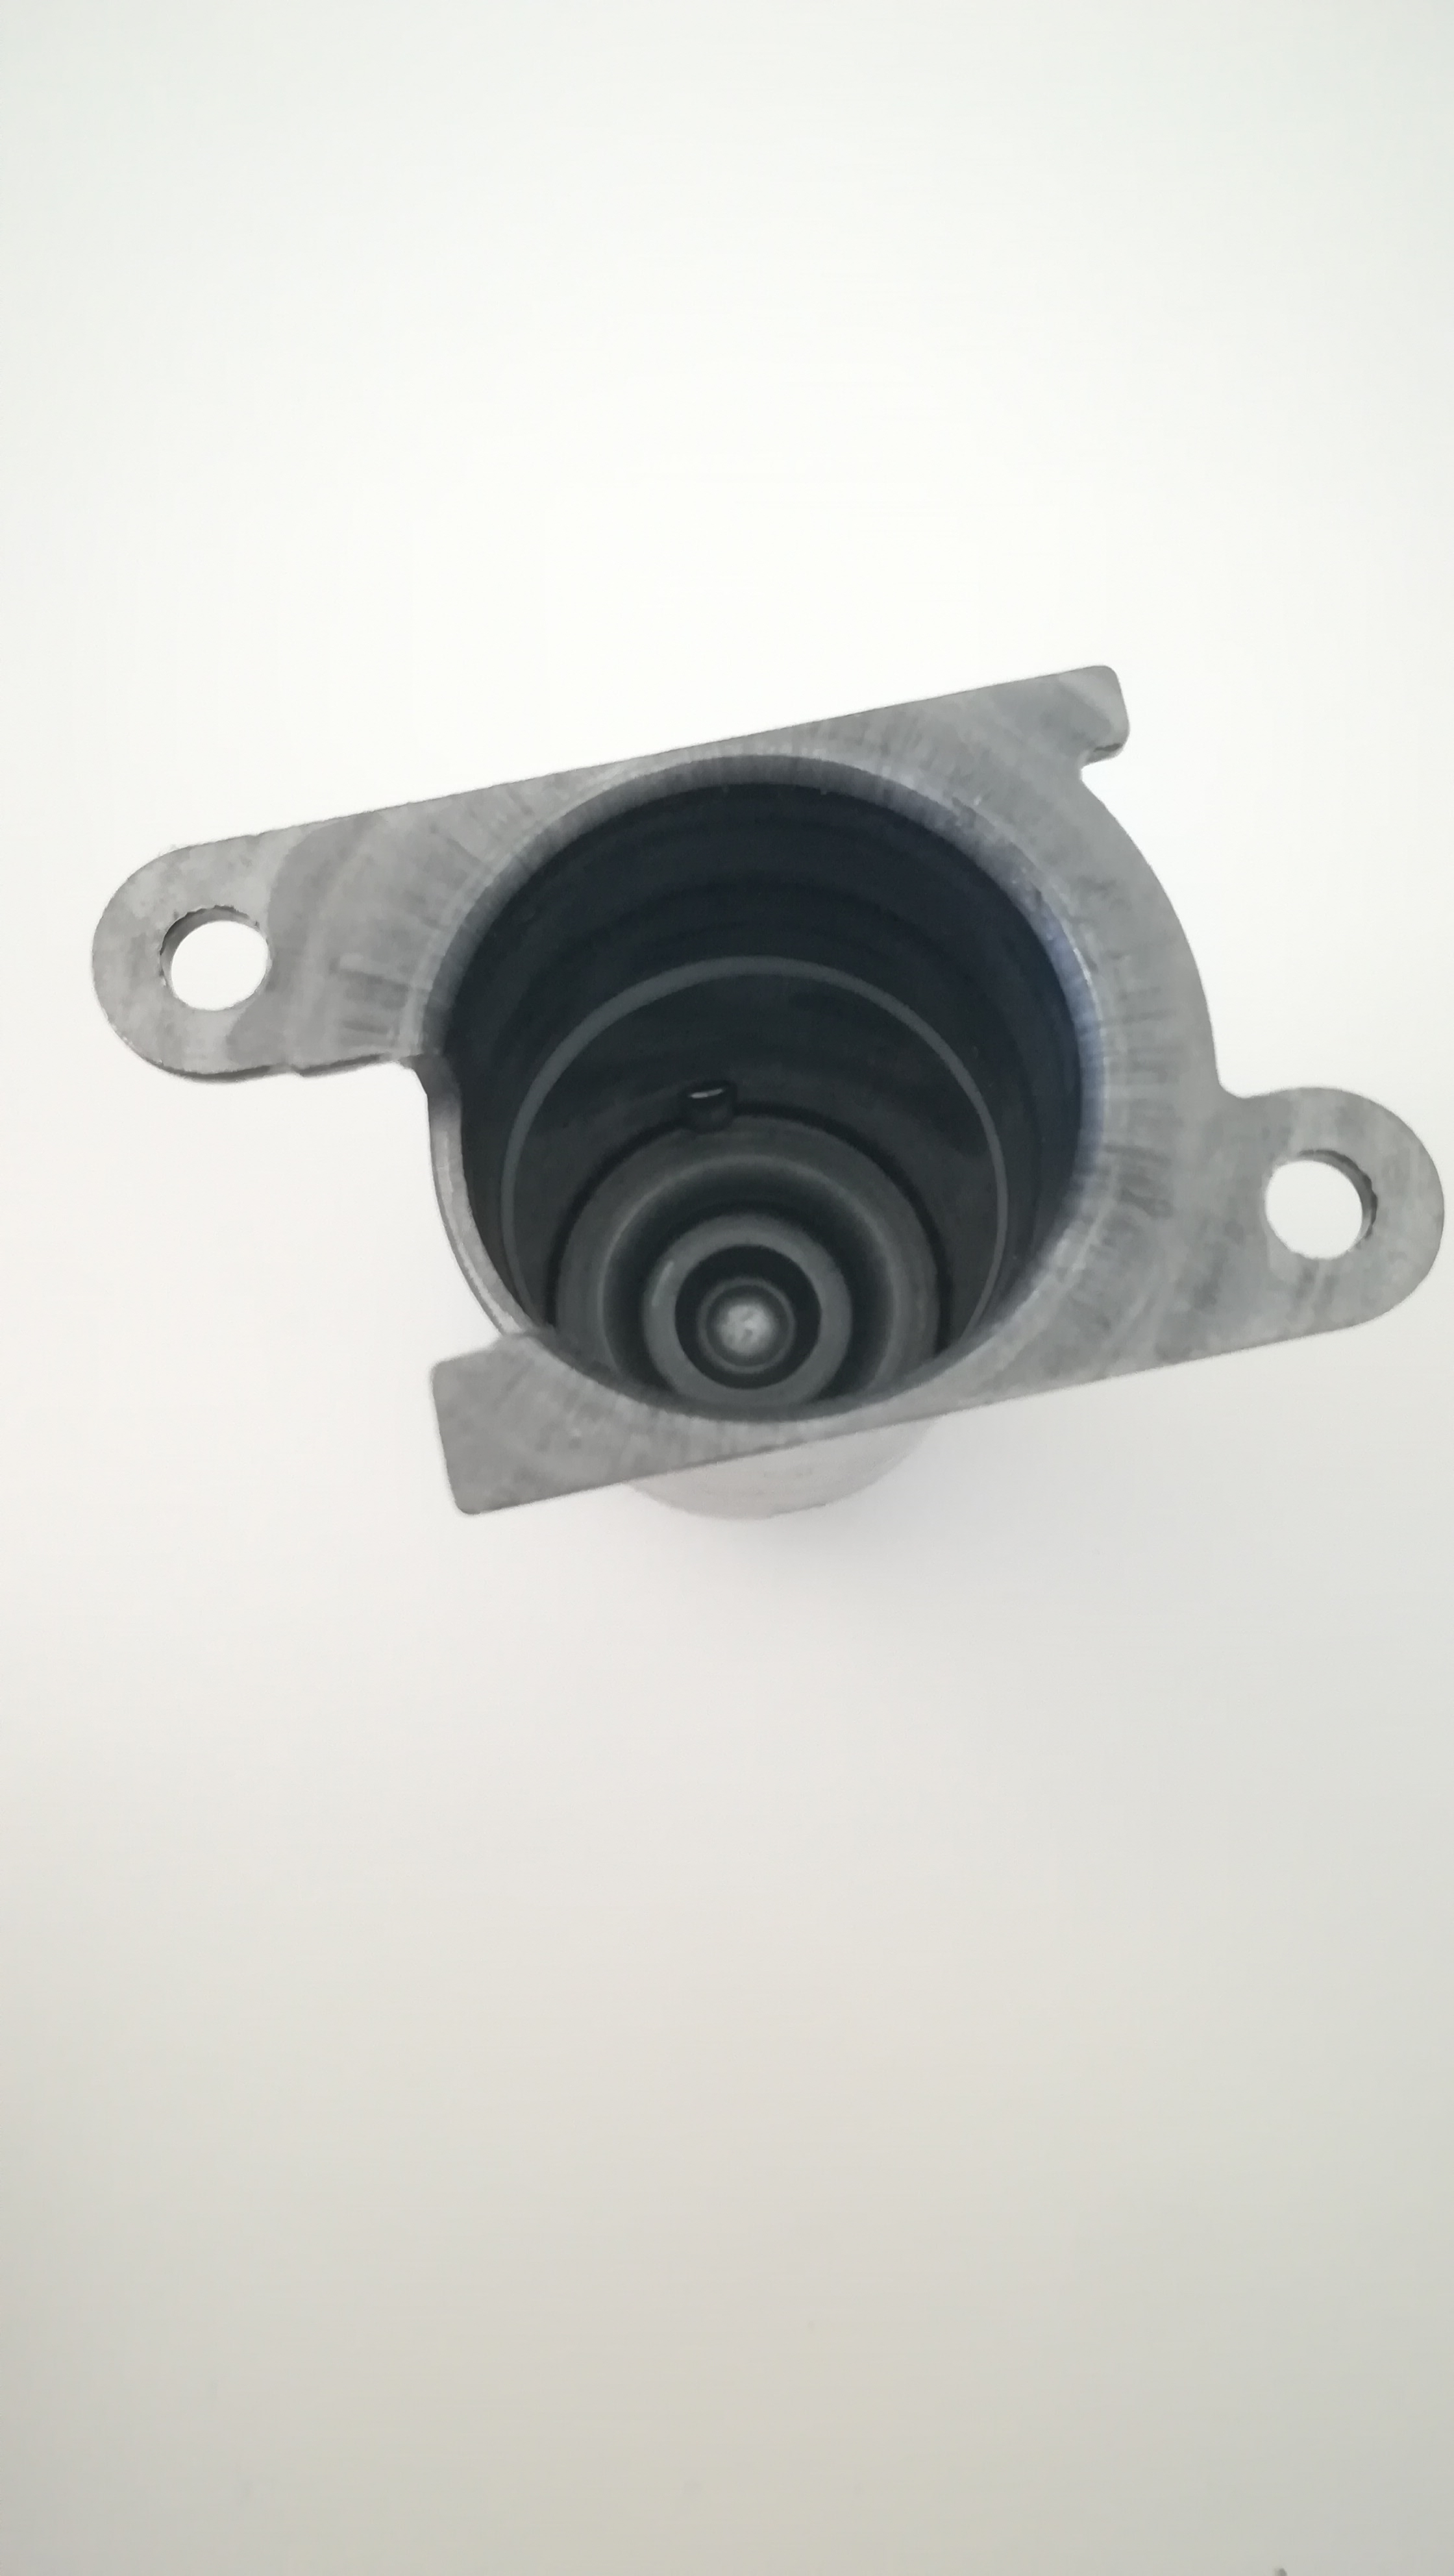
\includegraphics[width=3cm]{carcassa_da_sopra}
  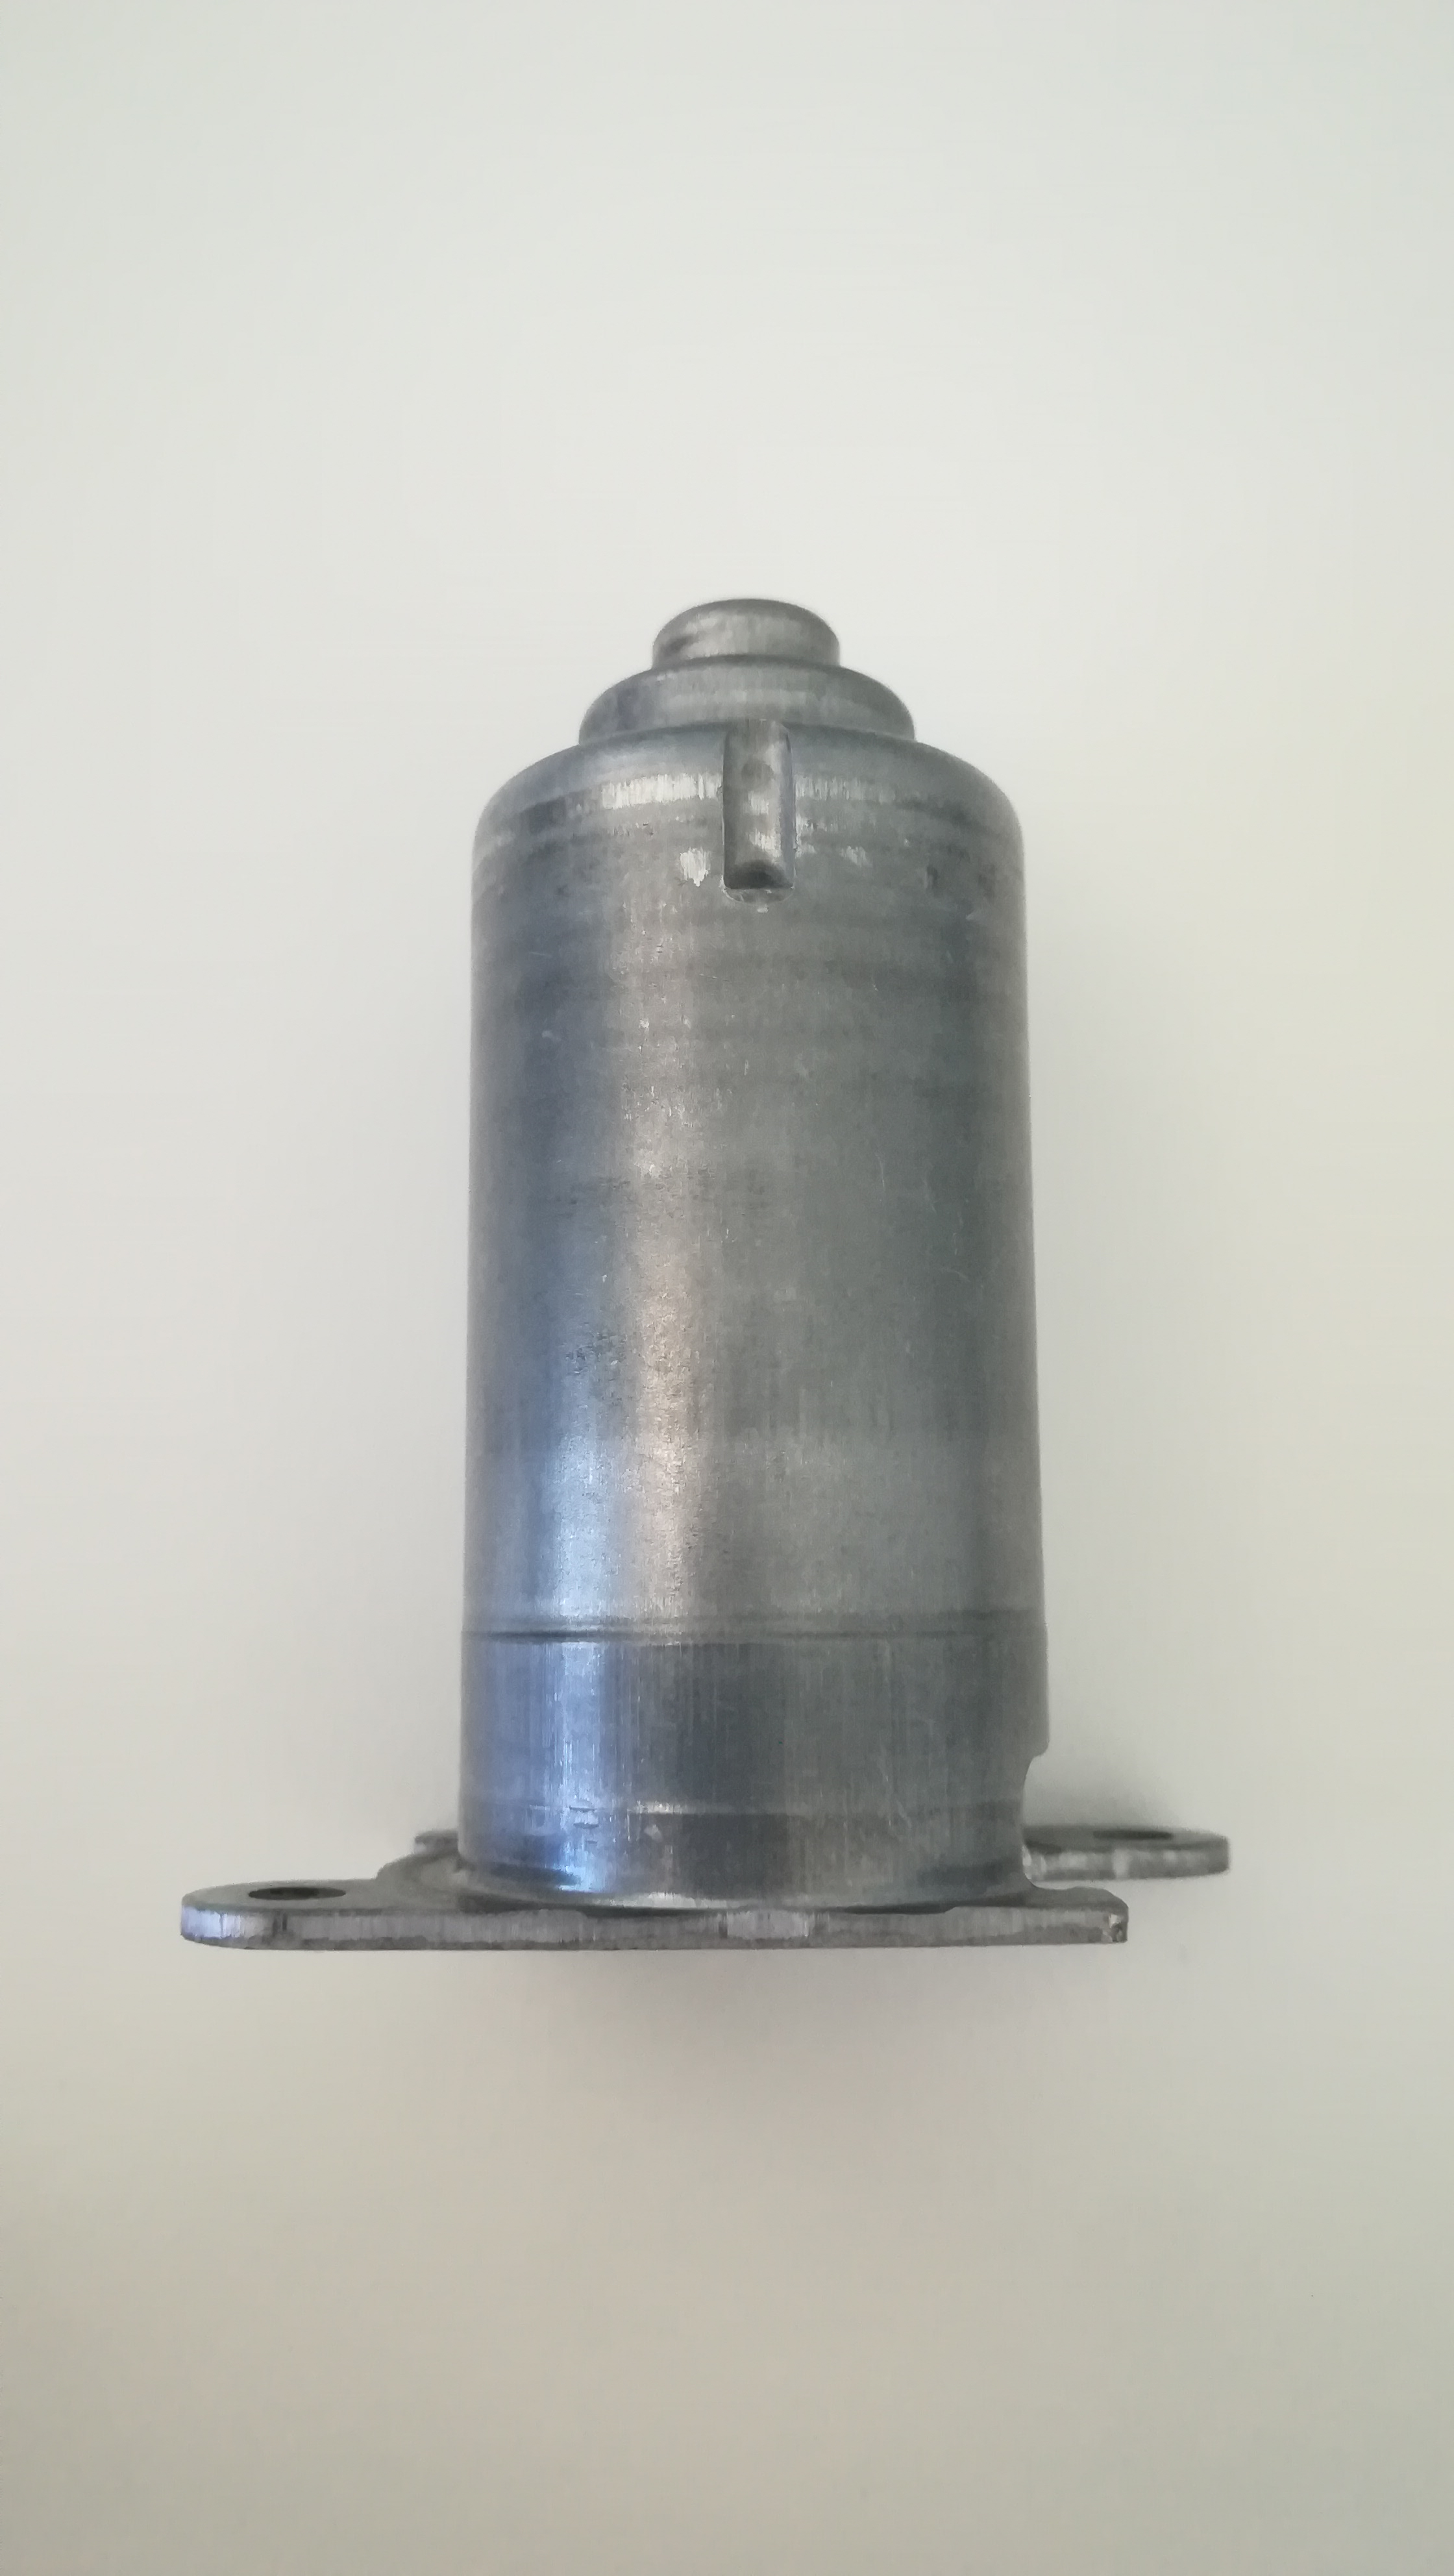
\includegraphics[width=3cm]{carcassa_di_lato}
  \caption{Visioni laterale e superiore di una carcassa}
  \label{fig:carc}
\end{figure}

Osservando le fotografie in figura, possono essere definite le caratteristiche principali delle carcasse:
\begin{itemize}
  \item il pezzo ha una struttura cilindrica cava;
  \item il fondo presenta tre gradini;
  \item sono presenti due balze (nella foto laterale se ne vede soltanto una), posizionate, una di fronte all'altra, prima del primo gradino;
  \item i supporti alla bocca della carcassa presentano due fori;
\end{itemize}
Il pezzo è stato pensato per avvolgere e proteggere motori elettrici.
Nello specifico i pezzi in foto, sui quali è stato svolto lo studio, sono carcasse per motori elettrici per tergicristalli.
I due fori aiuteranno a fissare con delle viti il pezzo su dei supporti in plastica.
Il motore alloggerà interamente nella cavità, nella quale verrà anche depositata della colla.
Questa verrà poi cotta in modo che il motore non possa vibrare all'interno della carcassa, evitando che eventuali urti possano danneggiarlo.
Dalla foto si può notare che la colla è distribuita in modo da formare un anello ad una altezza di circa $4cm$ dal fondo della carcassa.
La colla è stata depositata correttamente se:
\begin{enumerate}
  \item l'anello non presenta né sbavature né discontinuità;
  \item sul fondo non c'è presenza di colla.
\end{enumerate}
In questo documento, come si vedrà nella sezione sul \textit{dataset}, ci concentreremo esclusivamente sul secondo punto.
La presenza di colla sul fondo della carcassa causerà il malfunzionamento del motorino dopo un limitato tempo d'utilizzo, molto inferiore al tempo di vita atteso.
Per questo motivo è fondamentale che la colla venga depositata correttamente.


\section{Il Processo di Produzione}
Chiarire le modalità con cui le carcasse vengono manipolate, la colla viene depositata e le foto vengono acquisite risulta fondamentale.
Senza queste informazioni mancherebbe la base sulla quale costruire ipotesi e considerazioni riguardo le immagini del \textit{dataset}.
Analizzando le condizioni in cui le foto vengono scattate, si definiscono i vincoli ed i confini entro i quali le soluzioni proposte possono considerarsi verosimili ed applicabili al mondo reale.

Le carcasse, già presenti in grandi quantità in magazzino, raggiungono il macchinario e vengono caricate, con la concavità rivolta verso l'alto, su un disco rotante.
%TODO termini giusti sotto?
%TODO il processo è giusto?
Ad ogni ciclo macchina la colla, tramite due ugelli, viene depositata simultaneamente su due carcasse distinte.
Al contempo due sonde dotate di luce scendono nelle due carcasse su cui la colla era stata depositata il ciclo precedente, fino ad una distanza di circa $3cm$ dal fondo.
Le carcasse ritenute conformi procedono lungo un rullo trasportatore, mentre quelle che non idonee vengono scartate.

Vanno precisati vari aspetti.
Le carcasse, nonostante siano tutte dello stesso tipo, possono differire per quanto riguarda colore, graffi superficiali, sporco, incrostazioni oppure macchie.
Inoltre non vengono orientate tutte allo stesso modo rispetto all'asse verticale: questo ha delle ripercussioni dirette sulle foto raccolte, infatti le due balze non si presenteranno in posizioni fisse.

Il sistema assicura che le foto vengano scattate sempre alla stessa profondità e che la sonda sia centrata rispetto al pezzo (considerando come centro il centro della cavità cilindrica).
La distanza fissa è condizione sufficiente per garantire la messa a fuoco di ognuno dei tre gradini sul fondo.
Purtroppo non sono stati specificati dei vincoli riguardo l'illuminazione.

Si fa notare che il processo appena descritto viene eseguito da almeno due macchinari distinti, ovviamente questo aggiunge un ulteriore grado di sfida: non si può supporre che i macchinari siano sempre calibrati esattamente allo stesso modo.
%La nostra soluzione dovrà quindi essere in grado di resistere a TODO completare commento

In conclusione le foto che saranno da analizzare vengono raccolte da un totale di quattro fotocamere distinte, delle quali si assicura
\begin{itemize}
  \item con un grado di precisione soddisfacente la distanza dal fondo;
  \item con un grado di precisione accettabile la centratura delle immagini.
\end{itemize}
%TODO riassumere anche le caratteristiche delle carcasse?


\section{Gli Obiettivi da Raggiungere}
% TODO confrontarsi per veridicità
Di seguito sono riportati alcuni dati numerici riguardo i processi appena descritti.

La colla viene depositata su circa $5000$ pezzi al giorno, la probabilità che gocce di colla cadano sul fondo delle carcasse è estremamente bassa.
Purtroppo non esistono dati numerici esatti ma si stima che il macchinario abbia un \textit{fault rate} di una carcassa al mese o poco più.
Questi dati possono essere trasformati in probabilità approssimative osservando che:

\begin{center}
  \begin{tabular}{ l c r }
    colla depositata al mese: & $5000 * 31 =$& $155000$ \\
    colla mal depositata al mese: && $2$
  \end{tabular}
\end{center}
Quindi la probabilità che il macchinario sbagli e pari allo $0.00001\%$.
%Tenendo ben presente questa probabilità, si vorrebbe riconoscere, e quindi scartare, le carcasse che presentano colla sul fondo.
Il sistema di intelligenza artificiale deve riconoscere i pezzi non conformi ma soprattutto, tenendo conto della probabilità di cui sopra, deve generare un numero bassissimo di falsi positivi.
Ricordano che per falsi positivi (riferiti anche come FP o \textit{False Positive}) si intendono tutte le carcasse che il sistema considera non conformi ma che in realtà non presentano difetti.
Una AI troppo rigida, che, quando indecisa, propende per scartare il pezzo, inciderebbe negativamente sulla produzione.
Si rischierebbe, infatti di creare un enorme danno economico, andando a scartare molte più carcasse del necessario.
% usare teorema di bayes per dim che un modello aggressivo è peggio di uno che lascia passare

Il nostro obbiettivo è quindi quello di generare un numero di falsi positivi che sia inferiore al $2\%$, cercando di riconoscere più carcasse non conformi possibili.

% L'obbiettivo è riconoscere i pezzi che presentano colla sul fondo
% Acc sugli scarti $100\%$
% fp sui conformi $2\%$


% \section {L'attuale soluzione}
% " Tutti i vecchi metodi si arenavano causa differenze di tinta e luminosita' e rumorosita'"

%\cleardoublepage
% Riassunto sul dominio, obiettivi, strade già provate


%!TEX TS-program = pdflatex
%!TEX root = tesi.tex
%!TEX encoding = UTF-8 Unicode

\chapter{Il Dataset}

Innanzitutto si specifica che con la parola Scarto si indica l'immagine di una carcassa che presenta colla sul fondo, pezzo che, quindi, dovrà essere scartato.
Invece con la parola Conforme si indica l'immagine di una carcassa nella quale la colla è stata depositata correttamente, quindi con fondo pulito.

In questo capitolo verrà descritto il \textit{dataset} e gli algoritmi principali e la loro applicazione.
Si concluderà con la tecnica del data augmentation.
\todo{recap capitolo}


\section{Problematiche Principali}

\subsection{Dataset Piccolo e Sbilanciato}
La prima difficoltà insorge ancora prima di ispezionare le immagini del \textit{dataset}.
Infatti questo non solo comprende solamente 1749 immagini ma è anche fortemente sbilanciato:
\begin{itemize}
    \item 1719 immagini sono Conformi;
    \item 30 immagini sono Scarti.
\end{itemize}

A questo punto è corretto chiedersi se le quasi duemila immagini del \textit{dataset} siano sufficienti ai nostri scopi.
Nel campo del \textit{Machine Learning}, ed ancora di più in quello del \textit{Deep Learning}, non è raro che il numero di elementi in un dataset sia dell'ordine delle decine di migliaia se non di quello delle centinaia di migliaia.
Basti pensare ai dataset più famosi ed usati:
\todo{ aggiungere refs ai dataset con \cite{pyrl} }

\begin{itemize}
  \item MNIST è un dataset molto famoso contenente $70000$ cifre disegnate a mano appartenenti a $10$ classi in totale.
    È alla stesso tempo sia il punto di partenza dei principianti, perché di facile manipolazione, sia il campo di prova degli esperti, sul quale vengono allenati nuovi modelli prima di testarli su compiti più complessi.

  \item CIFAR-10 contiene $60000$ immagini a colori suddivise in 10 classi da 6000 immagini l'una.
    Le classi comprendono alcuni tipi di veicoli ed animali.
   Date le dimensioni ridotte delle immagini, appena $32$x$32$ pixel, il dataset occupa meno di $200 MB$, questo permette di allenare reti neurali in tempi ragionevoli.
    % https://www.cs.toronto.edu/~kriz/cifar.html

 \item ImageNet con i suoi 14 milioni di immagini è il più grande \textit{dataset} che sia mai stato creato.
    I più grandi esperti nel campo del \textit{Machine Learning} si sfidano annualmente su questo \textit{dataset}.
    Contiene decine di migliaia di classi e le sue immagini sono in gran parte fotografie scattate da volontari, che quindi hanno condizioni di luminosità e colori molti diversi tra loro.
    Possono variare anche la dimensione e l'orientamento, orizzontale o verticale, delle immagini.
    % https://en.wikipedia.org/wiki/ImageNet

\end{itemize}

Ciascuno di questi \textit{dataset} è stato etichettato\footnote{in inglese \textit{labeled} da \textit{label}, etichetta} a mano.
Ciò significa che ad ogni immagine è stata assegnata, a mano, una classe di appartenenza.
Prendendo in esempio MNIST, se un'immagine raffigura la cifra $7$ allora sarà etichettata con il \textit{label seven} ed apparterrà alla classe di immagini in cui compare la cifra $7$.
Allo stesso modo le immagini di ImageNet hanno etichette come \textit{dog}, \textit{cat}, \textit{bird}, \textit{car}, \textit{bike}, ecc\dots %TODO forma corretta??
%Il nostro contiene due classi: Conforme e Scarto.

Sembrerebbe che possedere 2000 immagini appena renda impossibile applicare algoritmi di \textit{Machine Learning}.
In realtà osservando i Conformi, in Figura \ref{fig:esempi_conformi} sono stati riportati alcuni esemplari significativi, ci si accorge che i pezzi sono molto simili.
Questo non ci sorprende, dato che i pezzi vengono generati meccanicamente, è perfettamente lecito supporre che nessuna carcassa abbia delle caratteristiche completamente differenti dalle altre.
Le principali diversità sono dovute ad imperfezioni superficiali come graffi o macchie.
Si può quindi dire che la distribuzione dei pezzi conformi è descritta bene anche da un numero limitato di esemplari.
Purtroppo il sistema di acquisizione immagini introduce ulteriori fattori di diversità come la posizione delle balze e la luminosità, ma questi fattori potranno essere gestiti senza troppe difficoltà.
Concludiamo che il numero di Conformi a nostra disposizione è sufficiente ai nostri scopi.

\begin{figure}[ht] % TODO
  \begin{center}
    \begin{tabular}{ccc}

  \begin{subfigure}{.3\linewidth}
    \centering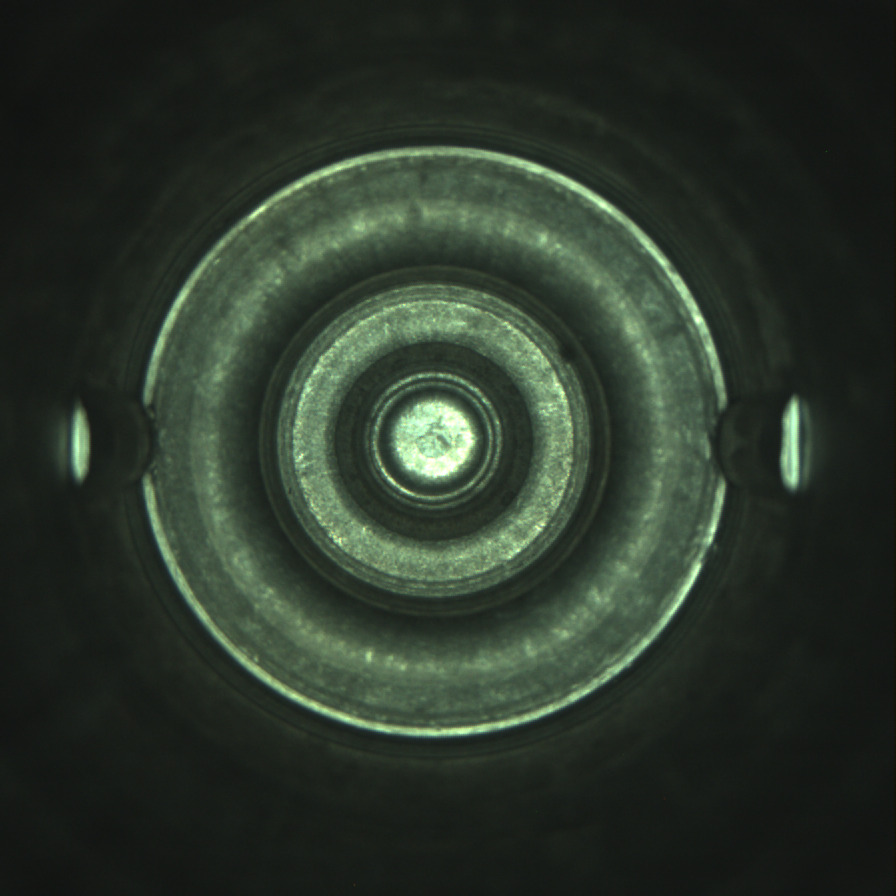
\includegraphics[width=\textwidth]{128___16760_0_0_1_OnLineAnalysis}
    \caption{}
  \end{subfigure} &

  \begin{subfigure}{.3\linewidth}
      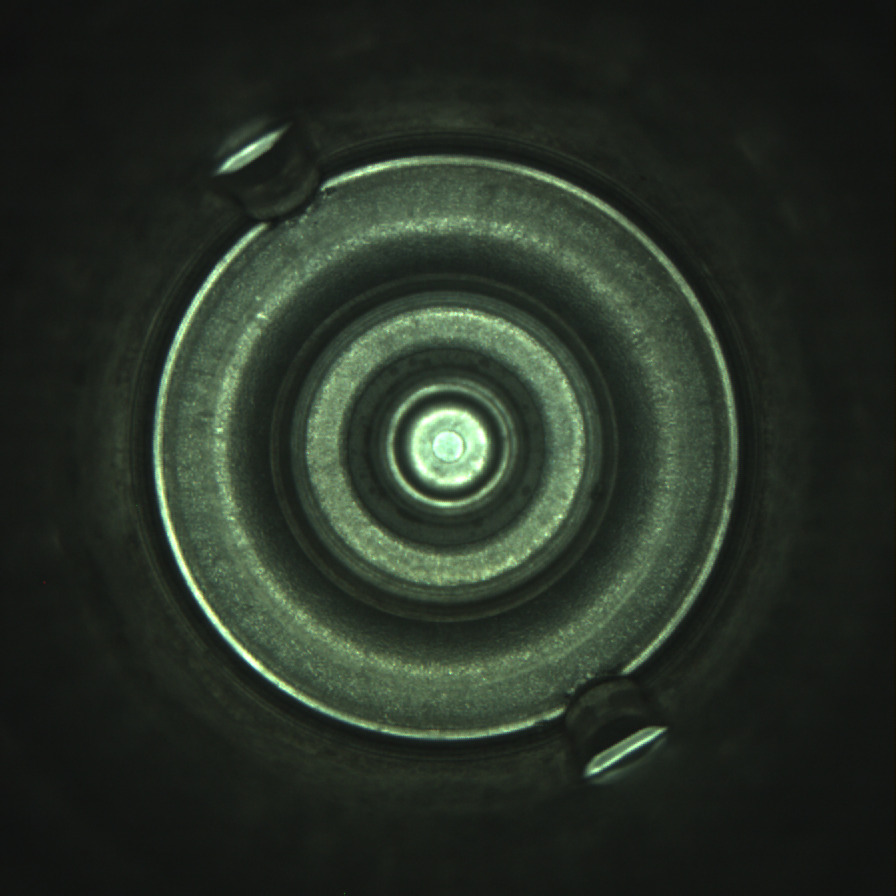
\includegraphics[width=\textwidth]{128___17986_1_1_1_OnLineAnalysis}
      \caption{}
    \end{subfigure} &

  \begin{subfigure}{.3\linewidth}
      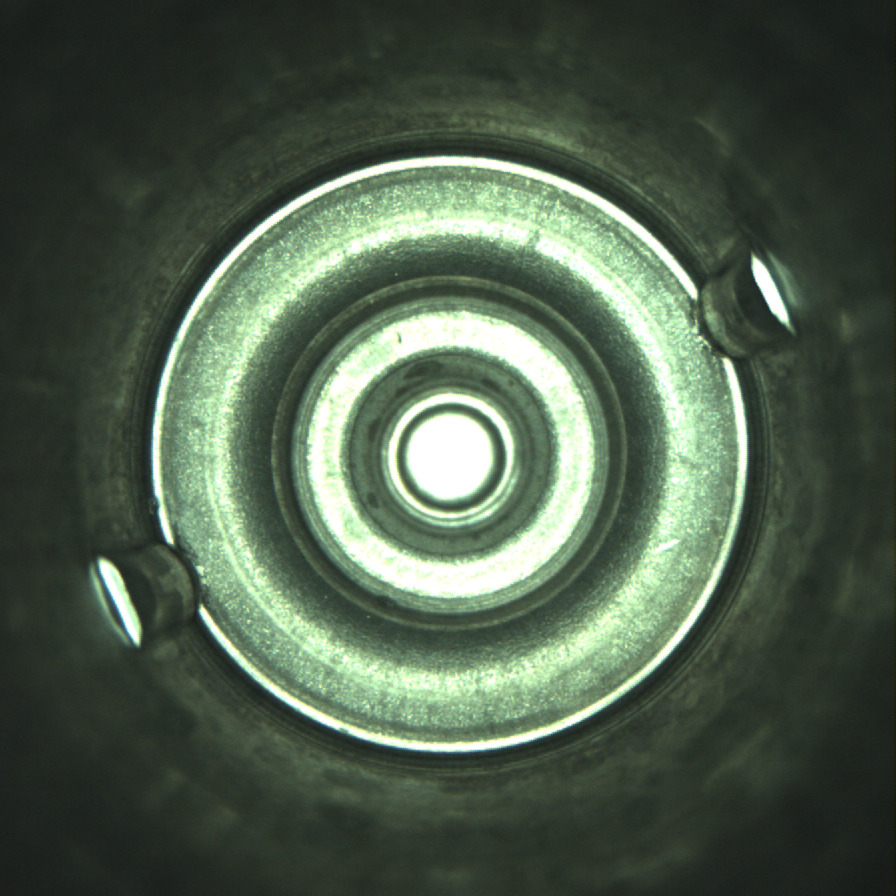
\includegraphics[width=\textwidth]{128___18037_1_0_1_OnLineAnalysis}
      \caption{}
    \end{subfigure} \\ \\

  \begin{subfigure}{.3\linewidth}
      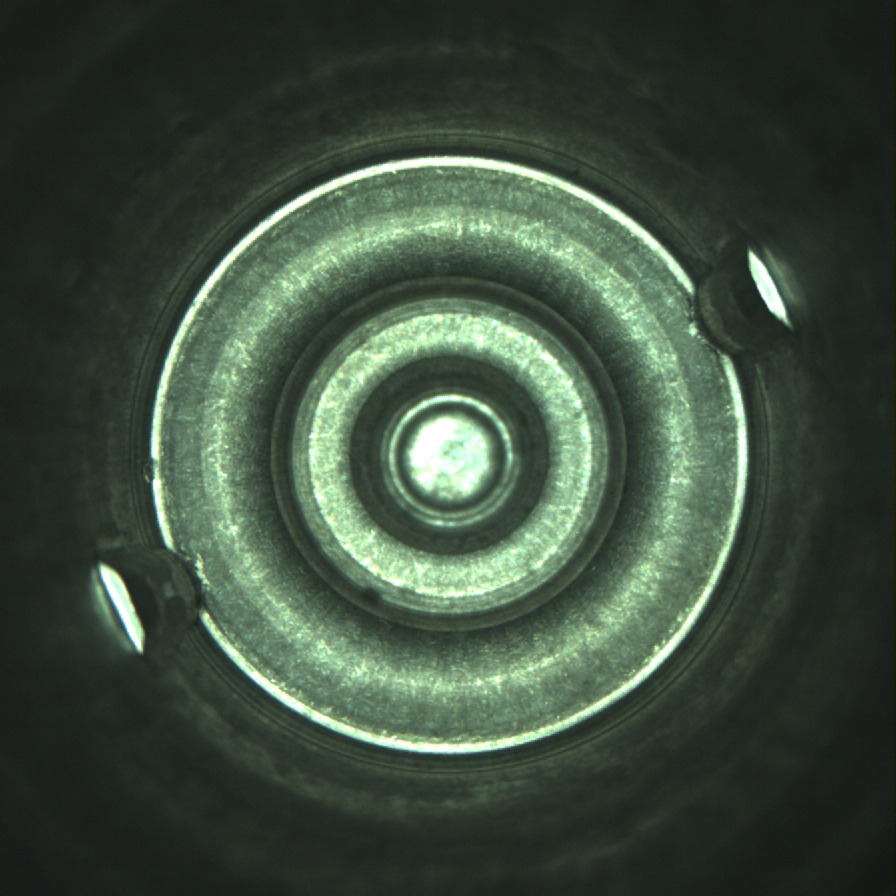
\includegraphics[width=\textwidth]{128___289_1_0_1_OnLineAnalysis}
      \caption{}
    \end{subfigure} &

  \begin{subfigure}{.3\linewidth}
      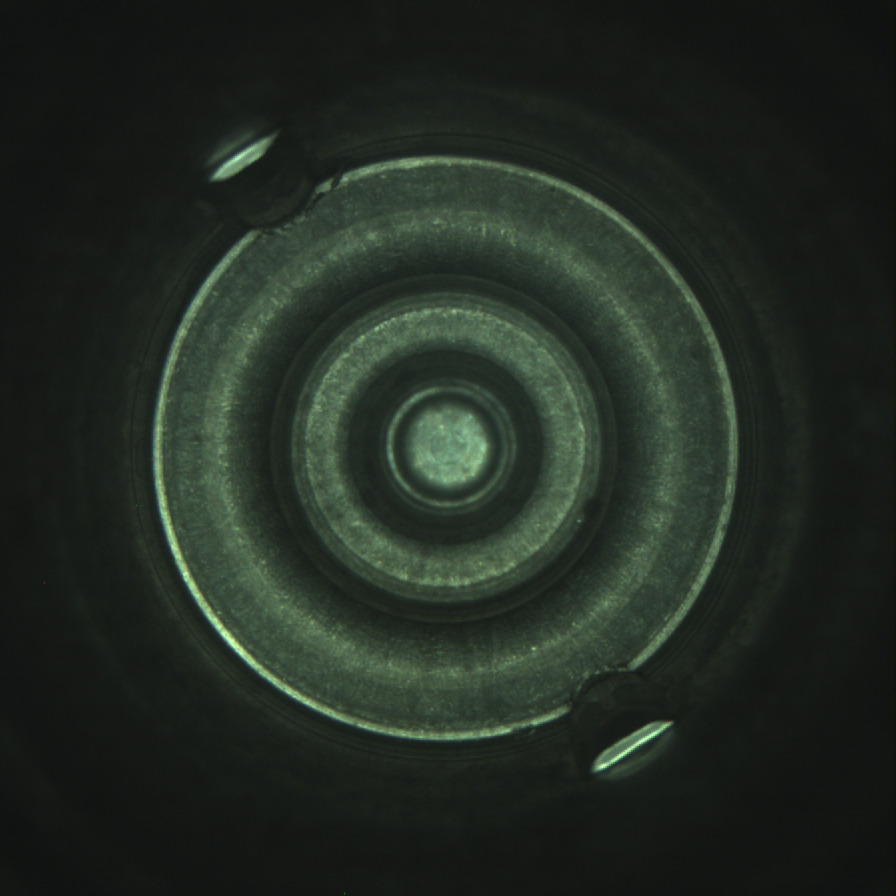
\includegraphics[width=\textwidth]{128___290_1_1_1_OnLineAnalysis}
      \caption{}
    \end{subfigure} &

    \begin{subfigure}{.3\linewidth}
      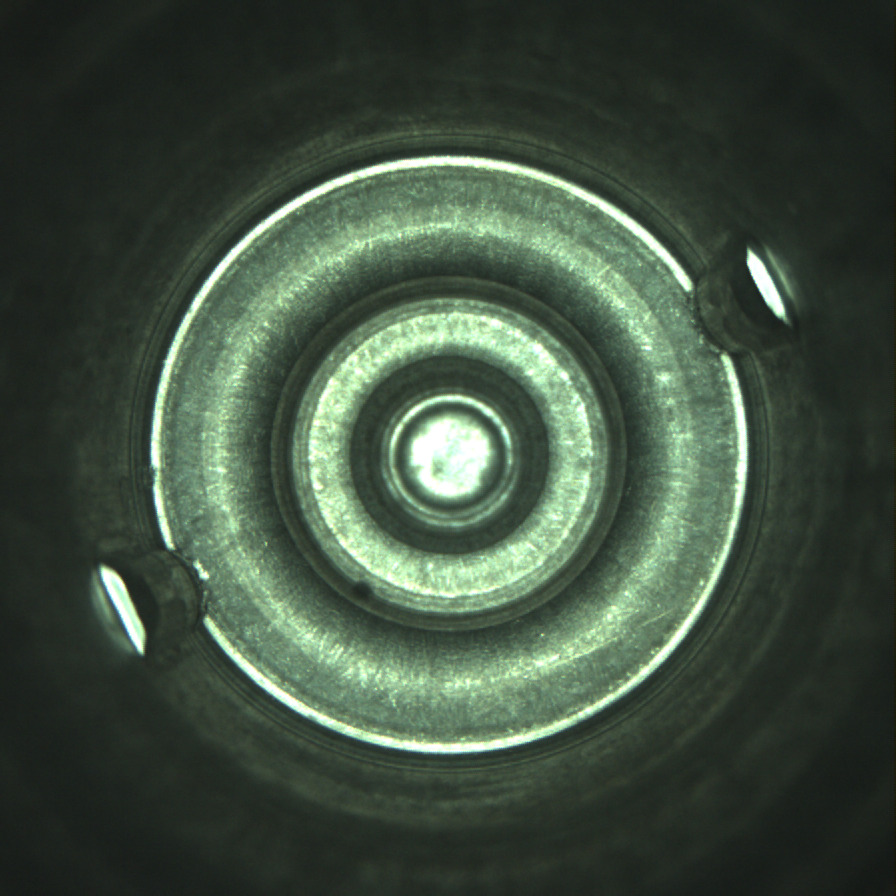
\includegraphics[width=\textwidth]{128___297_1_0_1_OnLineAnalysis}
      \caption{}
    \end{subfigure} \\

    \end{tabular}
    \caption{Alcune carcasse Conformi}
    \label{fig:esempi_conformi}
  \end{center}
\end{figure}

% https://tex.stackexchange.com/questions/333249/controlling-subfigure-captions-and-subfigure-placement

Non possiamo dire lo stesso per gli Scarti.
Se già la statistica ci lascia sospettare che $30$ esemplari non possono ritenersi significativi, allora questo sospetto diventa certezza quando si analizzano le caratteristiche della colla nelle immagini Scarto.  
Come si vede in Figura \ref{fig:esempi_scarti} la colla può presentarsi in forma di gocce più o meno circolari oppure come sbaffi di grossezza e lunghezza variabili.
Anche la quantità di superficie coperta dalla colla può variare notevolmente, passando da aree ridotte e localizzate ad aree estese e di conformazioni singolari.
Infine notiamo che la posizione del rimasuglio di colla all'interno della carcassa non è in relazione con la posizione delle balze e che la presenza dei gradini sul fondo non la obbliga in alcun modo a scivolare fino al centro.

\begin{figure}[ht] % TODO
  \begin{center}
    \begin{tabular}{ccc}

  \begin{subfigure}{.3\linewidth}
    \centering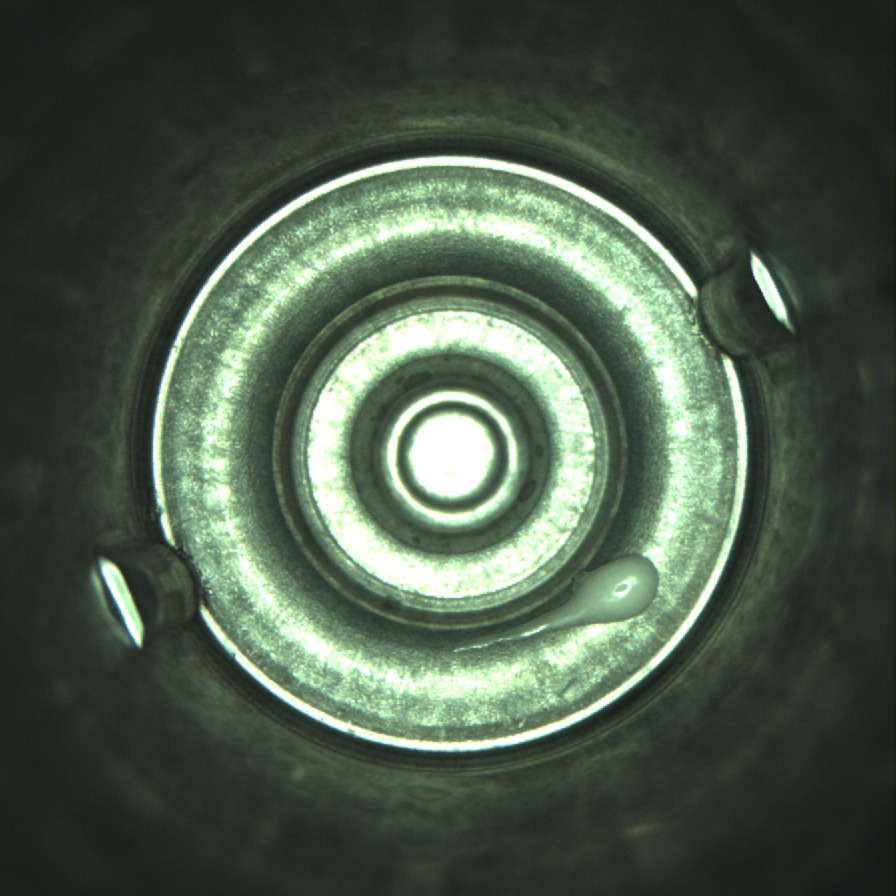
\includegraphics[width=\textwidth]{128___14097_1_0_1_OnLineAnalysis}
    \caption{}
  \end{subfigure} &

  \begin{subfigure}{.3\linewidth}
      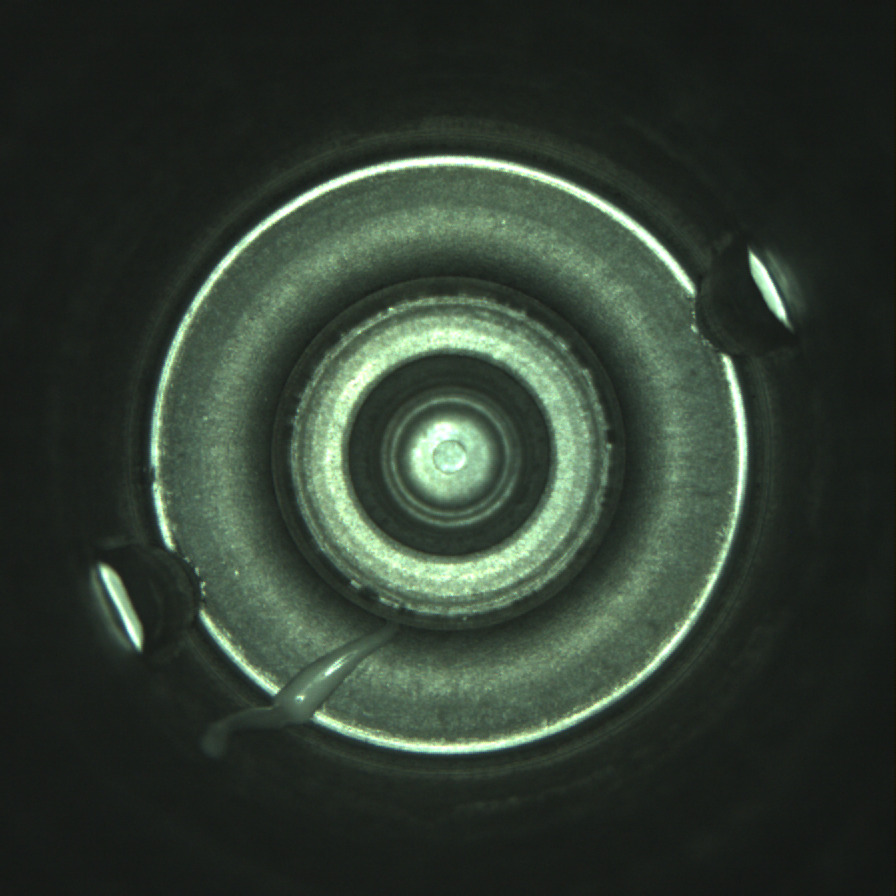
\includegraphics[width=\textwidth]{128___14177_1_0_1_OnLineAnalysis}
      \caption{}
      \label{fig:esempi_scarti_sbaffo}
    \end{subfigure} &

  \begin{subfigure}{.3\linewidth}
      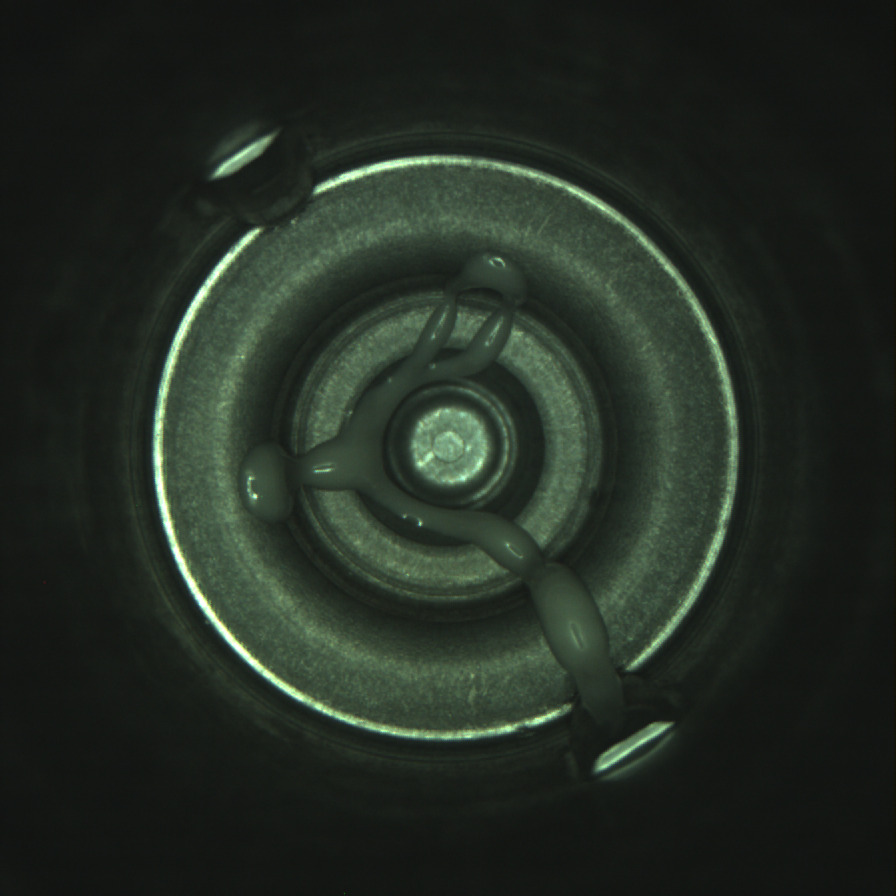
\includegraphics[width=\textwidth]{128___22886_1_1_1_OnLineAnalysis}
      \caption{}
    \end{subfigure} \\ \\

  \begin{subfigure}{.3\linewidth}
      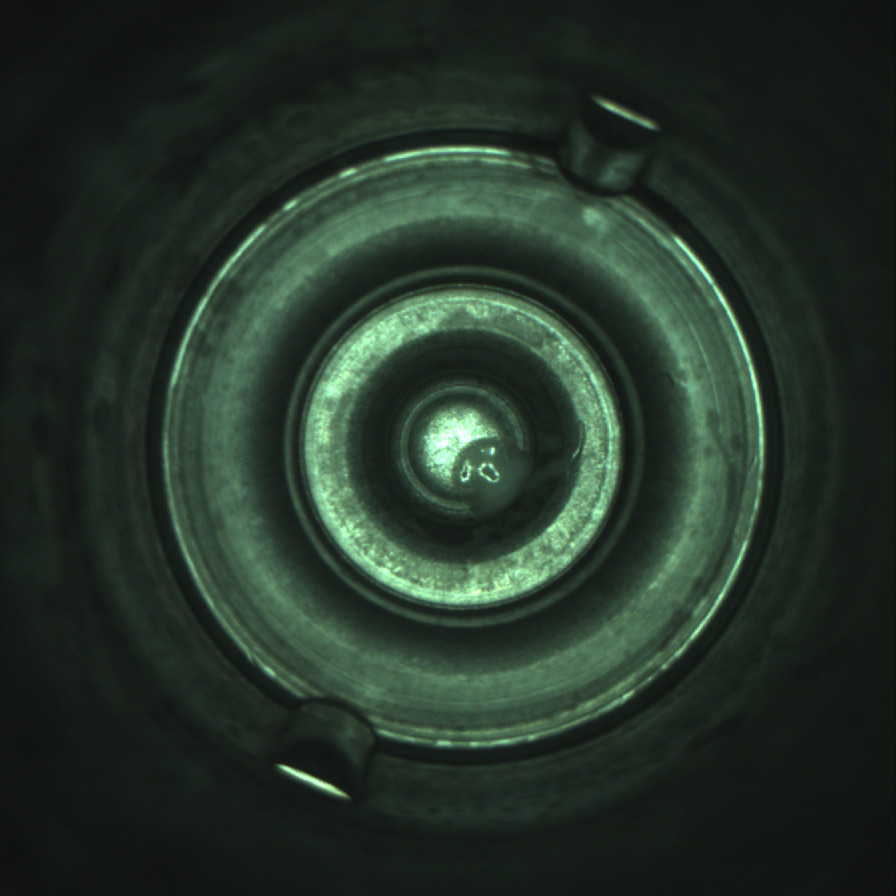
\includegraphics[width=\textwidth]{128___33657_0_0_1_OnLineAnalysis}
      \caption{}
      \label{fig:esempi_scarti_goccia}
    \end{subfigure} &

  \begin{subfigure}{.3\linewidth}
      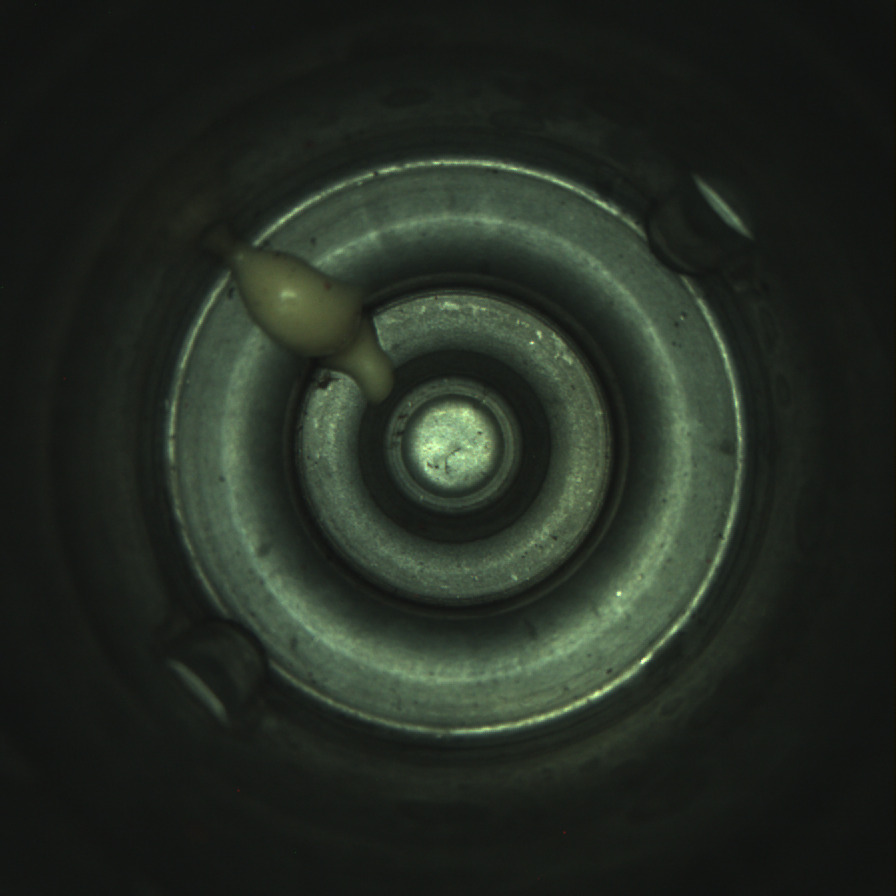
\includegraphics[width=\textwidth]{128___35_0_1_1_OnLineAnalysis}
      \caption{}
    \end{subfigure} &

    \begin{subfigure}{.3\linewidth}
      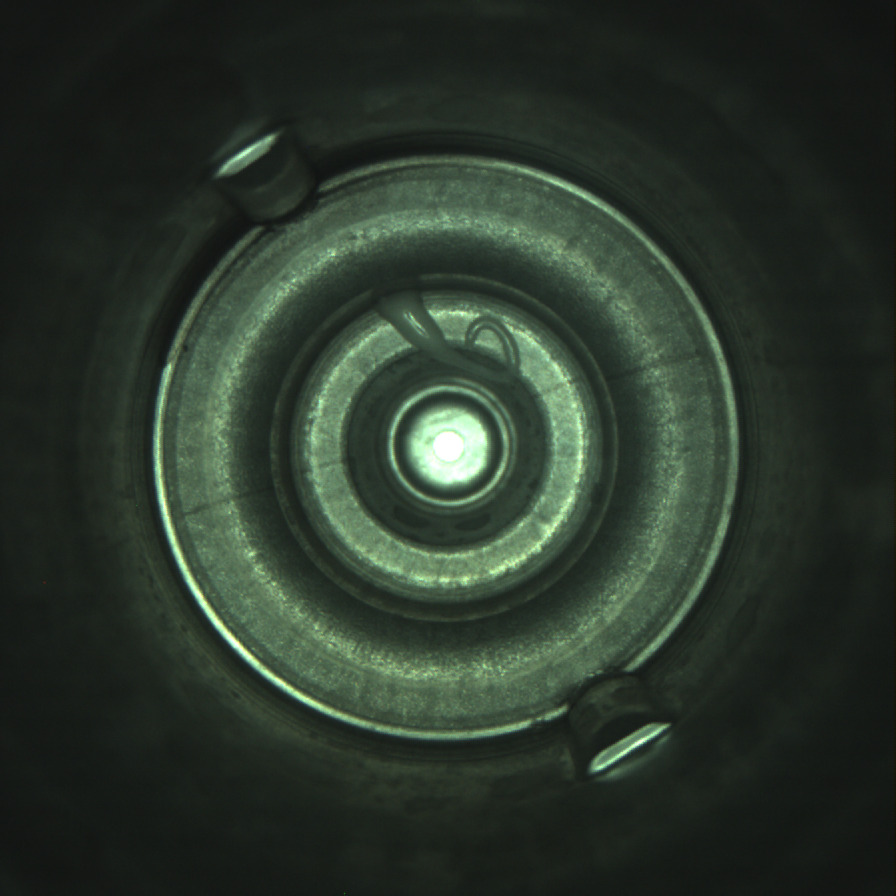
\includegraphics[width=\textwidth]{128___5668_1_1_1_OnLineAnalysis}
      \caption{}
    \end{subfigure} \\

    \end{tabular}
    \caption{Alcune carcasse Scarto}
    \label{fig:esempi_scarti}
  \end{center}
\end{figure}

Per analizzare meglio le modalità con cui potrebbe essere generato uno Scarto si supponga che il macchinario abbia commesso un errore: dall'ugello è uscita un certa quantità di colla in esubero.
A seconda della posizione dell'ugello rispetto alla carcassa si può immaginare che la colla raggiunga il fondo in vari modi, proviamo ora ad illustrarne due:
\begin{itemize}
  \item nel primo caso si immagina che il braccio abbia già depositato l'anello di colla e che si stia allontanando dalla carcassa.
    La colla in esubero cadrebbe sotto forma si goccia fino a raggiungere il fondo del pezzo.
    Questo potrebbe esse il caso per la Figura~\ref{fig:esempi_scarti_goccia};
  \item nel secondo caso si ipotizza che la colla in esubero faccia parte dell'anello appena depositato e che, a causa delle vibrazioni o di altri fattori simili, coli raggiungendo il fondo della carcassa.
    Questo potrebbe esse il caso per la Figura~\ref{fig:esempi_scarti_sbaffo}.
\end{itemize}

Data la grande varietà di modi in cui la colla può presentarsi, concludiamo che gli esemplari forniti per la classe Scarto la descrivono soltanto in modo parziale.
Ciò rappresenta la maggiore difficoltà del \textit{dataset}, infatti è risaputo che ogni tecnica di \textit{machine learning} richiede che i dati racchiudano tutte le informazioni per poter generalizzare correttamente tutti i dati futuri. \todo{ref a documento in cui si spiega l'importanza del dataset}

la distribuzione della classe \todo{dire meglio} e che quindi non possono essere utilizzati per allenare un modello veramente generale.

Infatti se, per esempio, venissero usati per il train di una rete convolutiva, di cui poi verrà illustrata brevemente la struttura, si rischierebbe di creare un modello con forte \textit{overfit} rispetto a quelle specifiche macchie di colla fornite.
\todo{definire overfit}
%Dopo queste osservazioni siamo convinti che il problema deve essere affrontato com e un problema di anomaly detection... Piccola introduzione? Meglio parlarne vicino agli AE

Prima di proseguire con le prossime problematiche dobbiamo spendere alcune parole per commentare la colorazione delle immagini rispetto ai veri colori delle carcasse e della colla.
In figura~\ref{fig:carc} a pagina \pageref{fig:carc} abbiamo visto che la superficie del pezzo è di colore grigio ma nella foto risulta di colore verdastro.
Allo stesso modo anche la colla, in realtà di colore bianco sporco, nella fotografia assume tonalità verdognole.
Per certi compiti possedere immagini in falsi colori può risultare problematico ma fortunatamente non è questo il caso: l'importante è che venga mantenuta l'informazione che ci permette di distinguere la colla dalla superficie della carcassa.
Come vedremo poi le immagini verranno trasformate in scala di grigi quindi, nonostante sarebbe stato preferibile avere immagini a colori reali, i falsi colori non sono da considerarsi problematici.

\subsection{Differenze tra Immagini}
Ora che abbiamo una visione d'insieme sul dataset possiamo concentrare la nostra attenzione sulle proprietà principali delle immagini.
Innanzitutto ogni immagine ha una risoluzione di $896$x$896$ pixel, dimensione che ci permette di esplorare varie possibilità.
Ad esempio si può pensare di ridurre l'immagine ad una dimensione tale da: occupare meno spazio in memoria, quindi in RAM durante l'allenamento della rete, ed allo stesso tempo di mantenere un livello di dettaglio sufficiente ai nostri scopi.
Oppure di suddividere l'immagine in quadranti da analizzare singolarmente così da mantenere la qualità dell'immagine originale ma senza dover creare una rete che accetti immagini troppo grandi.
Infatti una rete che prende in input immagini di grandi dimensioni, solitamente, avrà un numero di parametri maggiore di una che accetta immagini piccole.
Questo porta non solo ad occupare più spazio in memoria ma significa anche che la rete impiegherà più tempo in fase di \textit{train}, perché dovrà impostare correttamente un maggior numero di parametri.
Per avere un termine di paragone basti pensare che le immagini di MNIST sono $64$x$64$ pixel mentre quelle di ImageNet, che ricordiamo hanno dimensioni variabili, vengono solitamente scalate a $224$x$224px$. \todo{ref a documento}

%% falsi colori, contrasti differenti, centramenti
Osservando nuovamente Figura \ref{fig:esempi_conformi} ci si accorge che le immagini hanno varie proprietà.
Verranno ora elencate a partire da quella da considerarsi meno problematica fino ad arrivare a quella più problematica.
\begin{itemize}

  \item Ogni immagine presenta tre circonferenze concentriche, con centro il centro del pezzo.
    Ciascuna circonferenza è definita da una transizione da una zona più scura ad una più chiara.
    Sappiamo che le zone più scure corrispondono alle pareti verticali del pezzo mentre le zone chiare ai tre gradini sul fondo.
    Questa proprietà non è problematica, anzi potrà essere sfruttata a nostro vantaggio.

  \item Dato che le immagini vengono raccolte ad una distanza costante dal fondo, la dimensioni delle circonferenze sono fissate e si mantengono coerenti tra le immagini. Anche questa proprietà verrà usata a nostro vantaggio.

  \item Le due balze sulla parete verticale sono ben visibili e possono presentarsi, sempre una di fronte all'altra, in ogni posizione lungo una circonferenza di raggio pari al raggio della cavità cilindrica.
    Possono essere considerate un problema in quanto rappresentano informazione superflua e variabile.
    Ricordiamo che la posizione delle balze non ha alcuna correlazione con la presenza della colla, tanto meno con la sua posizione.

  \item Le superfici dei pezzi si assomigliano: presentano tutte un effetto chiamato "sale e pepe" con granuli di grandezze e luminosità varia.
    %Questo è un bene perché è una costante ma anche un male perché ognuno ha una particolare disposizione di quella texture. TODO dire meglio.
    Bisogna prestare particolare attenzione alle macchie scure presenti sul fondo di alcune carcasse.
    La posizione delle macchie non è fissa, perdipiù anche la loro dimensione è variabile.
    Queste qualità superficiali non saranno da sottovalutare in fase di elaborazione delle immagini.

  \item Ad un primo sguardo potrebbe sembrare che le immagini siano tutte centrate allo stesso modo, invece in molte il centro dell'immagine non corrisponde con il centro del pezzo.
    Nonostante la distanza massima tra centro del pezzo e centro dell'immagine è tale che il fondo della carcassa sia sempre visibile interamente, è preferibile che le carcasse vengano centrate correttamente.\todo{dire meglio}
  
  % TODO decidere se metterlo
  %\item La luminosità del gradino più piccolo, quello al centro dell'immagine, varia di molto.
  %  Questo comporta un problema perché in alcune immagini con luminosità maggiore il cerchio più piccolo risulta completamente bianco.
  %  Se lo confrontiamo con un'altra immagine si vede che sono state perse tutte le informazioni sulla superficie del fondo. (TODO dire meglio).
  %  Questo sarebbe una problematica secondaria se non fosse che la colla può colare fino al centro.
  %  Poiché la colorazione della colla è nell'intorno del bianco bisognerà trovare un modo per smorzare la luminosità del fondo.

  \item La variazione di luminosità tra le varie foto è una problematica che dovrà essere assolutamente gestita.
    Infatti alcune immagini hanno una luminosità così alta da far risultare alcune superfici bianche.
    Altre immagini, invece, sono molto più scure, tanto che anche le zone che normalmente rifletterebbero sono illuminate appena.

\end{itemize}

% TODO 3 immagini conformi vicine il più diverse possibile??
Ora, facendo riferimento alla Figura \ref{fig:esempi_scarti}, possiamo elencare le proprietà esclusive degli Scarti.
In questo caso sono tutte non problematiche, anzi sono sfruttabili poiché rappresentano informazione con cui si può distingue uno scarto da un conforme:
\begin{itemize}
  \item La colla ha alcune caratteristiche particolari: ha un colore bianco-verde solitamente più chiaro della superficie della carcassa e presenta sempre delle zone con dei riflessi.

  \item La colla è localizzata.
    Significa che, se presente, non appare come tante gocce sparse ma come un corpo unico più o meno allungato.

  \item Tracciando una diametro a piacere ci si accorge che gli Scarti sono sempre asimmetrici, invece i conformi, a meno di piccole differenze superficiali, sono sempre simmetrici. % (TODO dire meglio).

\end{itemize}


% TODO manca qualcosa?
% TODO fare conclusione section/subsection?

\clearpage
\section{Pre-Processing}
Questa sezione è divisa in due parti: nella prima verranno illustrate alcune tra le principali tecniche di \textit{Digital Image Processing} nonché di \textit{Computer Vision}, esponendo i dettagli matematici ed esplorando le loro applicazioni; nella seconda si spiegherà quali di queste tecniche, in che ordine e per quali motivi sono state utilizzate.
\todo{TODO Descrivere cose'è preprocesing resto(DIP, Machine e Compute Vision) lasciamolo all'introduzione}

Come prima cosa è bene ricordare che con \textit{Digital Image Processing} si intende il modificare immagini digitali per mezzo di algoritmi eseguibili da un calcolatore.

TODO descrivere pre-processing anziché Digital Image Processing?(Il DIP nelle altr sezioni o mai)
Il pre-processing è il manipolare le immagini digitali per renderle utilizzabili da altri algoritmi, nel nostro caso si manipoler

Gli algoritmi utilizzati in questi campi hanno precise formulazioni matematiche perché ogni immagine viene rappresentata come una matrice bidimensionale, se in scala di grigi, oppure tridimensionale se a colori.
Gli elementi di una matrice bidimensionale appartengono all'intervallo $[0,255]$, nel quale $0$ corrisponde al colore nero mentre $255$ corrisponde al bianco.
Disponendo una sopra l'altra tre matrici come quelle appena descritte si ottiene un'immagine a colori: ogni matrice rappresenta uno dei canali principali (Red, Green, Blue da cui il famoso acronimo RGB) dell'immagine.
Sia $I$ un'immagine a tre canali (RGB), il colore del pixel in posizione $(i,j)$ è dato dalla tripletta $(I[i,j,0], I[i,j,1], I[i,j,2])$, in cui: $(0,0,0)$ indica il colore nero, $(255,255,255)$ indica il colore bianco, $(255,0,0)$ indica il colore rosso, $(0,255,0)$ indica il colore verde, e così via \dots
Quindi un'immagine avrà un numero finito di elementi, detti \textit{pixel}, il cui numero si può ottenere moltiplicando il numero di colonne della matrice per il numero di righe.
% potrei definire qua lo aspect ratio

% La definizione di immagine appena data prende il nome di \textit{raster-image}.
% https://en.wikipedia.org/wiki/Raster_graphics

Uno dei vantaggi del rappresentare le immagini come matrici è quello di poter applicare operazioni classiche come somma, sottrazione, prodotto e divisione.
Ma la nostra attenzione si concentrerà soprattutto sulle convoluzioni.

Nell'ambito del \textit{Image Processing} con convoluzione si intende l'operazione che permette di effettuare, per ogni pixel dell'immagine, una somma pesata tra il pixel e gli elementi a lui vicini.
I pesi sono definiti in una matrice, detta \textit{kernel} o filtro, di dimensioni non superiori a quelle dell'immagine di partenza.
Solitamente i kernel hanno dimensione $3x3$ o $5x5$.%\todo{ref alla risorsa?}
Una convoluzione è composta da semplici passi.
Prima il filtro viene centrato su un pixel.
A questo punto è come se il kernel coprisse un'area quadrata dell'immagine: moltiplichiamo i valori dei pixel con i rispettivi valori del filtro.
I prodotti così ottenuti dovranno essere sommati assieme, il risultato della somma sarà il nuovo valore del pixel su cui il kernel era stato centrato.
Effettuiamo questa operazione per ogni elemento dell'immagine.
Si fa presente che di solito le convoluzioni si effettuano da sinistra a destra e dall'alto verso il basso, ma si fa presente che l'ordine d'esecuzione non deve modificare il risultato.
Infatti è importante aggiornare i pixel solo dopo aver ottenuto i nuovi valori dei pixel di tutta l'immagine.

%\paragraph{Feature Extraction}
Prima di cominciare a descrivere gli algoritmi, si vuole specificare cosa significa \textit{Feature Extraction}.
\todo[noline]{completare}
In generale indica un procedimento con cui si estrapolano, da un'insieme di dati formato,  un sottoinsieme ...


% https://en.wikipedia.org/wiki/Feature_extraction
% https://deepai.org/machine-learning-glossary-and-terms/feature-extraction

\clearpage
Ora verranno introdotti alcuni algoritmi fondamentali nel campo della \textit{Computer Vision}.
\todo{TODO machine o computer?}

% TODO aggiungere applicazioni principali per ogni tecnica?
% TODO sono da riscrivere meglio.


\subsection {Passaggio da RGB a GrayScale}
La conversione di un'immagine da RGB in scala di grigi è un'operazione estremamente facile, ma rimane comunque alla base di molti algoritmi di image processing.
Infatti per molti compiti l'informazione sul colore non è necessaria.
Il modo più semplice per combinare i tre canali RGB in un unico canale è quello di fare la media dei valori pixel per pixel:
\begin{equation}
  Y = (R + G + B)/3
\end{equation}
\label{eq:rgb2gray_avg}
In questo modo ogni canale partecipa allo stesso modo.
Però sappiamo che l'occhio umano è più sensibile ai colori verdi, quindi potrebbe essere preferibile dare più importanza al secondo canale:
\begin{equation}
  Y = 0.299*R + 0.587*G + 0.114*B
\end{equation}
\label{eq:rgb2gray}
I pesi sono stati definiti nello standard CCIR 601.
Il risulato di quest'ultimo calcolo è rappresentato in Figura~\ref{fig:rgb2gray_example}.

% TODO accennare agli altri metodi?
% https://www.johndcook.com/blog/2009/08/24/algorithms-convert-color-grayscale/
% https://docs.opencv.org/3.1.0/de/d25/imgproc_color_conversions.html
% https://stackoverflow.com/questions/19181323/what-grayscale-conversion-algorithm-does-opencv-cvtcolor-use
\begin{figure}[ht]
  \begin{center}
    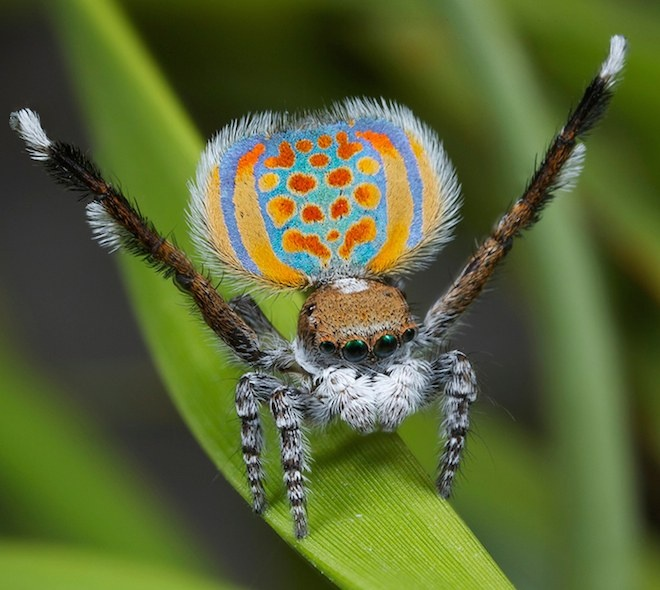
\includegraphics[width=0.4\textwidth]{RGB}
    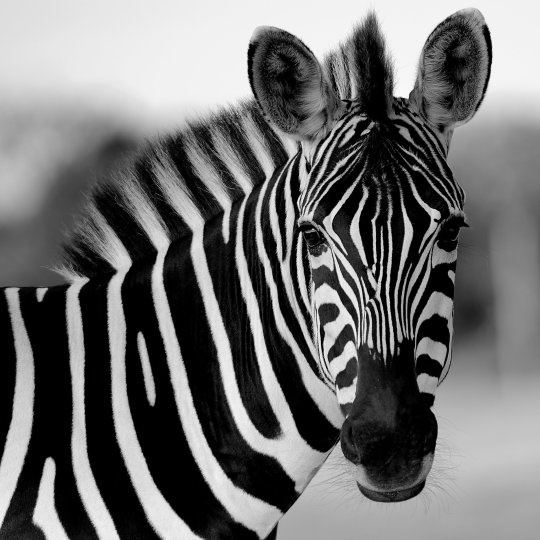
\includegraphics[width=0.4\textwidth]{RGBtoGRAY}
    \caption{A sinistra l'immagine originale. A destra la versione in scala di grigi}
    \label{fig:rgb2gray_example}
  \end{center}
\end{figure}


\clearpage
\subsection {Masking}
La tecnica del masking permette di nascondere parti di immagine a cui non siamo interessati.
Abbiamo bisogno di una maschera binaria, nella quale ogni pixel appartiene all'insieme $\{0,1\}$, che solitamente viene generata a mano, ed ovviamente dell'immagine che si vuole mascherare.
La maschera deve avere le stesse dimensioni dell'immagine di partenza.
L'operazione consiste nell'effettuare un AND logico, pixel per pixel,  tra l'immagine e la maschera.
Così facendo tutti i pixel dell'immagine di partenza corrispondenti a zone di valore $0$ della maschera verranno impostati a $0$, diventando quindi neri.
Il resto dell'immagine rimane con i colori originali.

Nell'esempio in Figura~\ref{fig:mask_example} si è deciso di rimuove l'informazione relativa allo sfondo.
\begin{figure}[ht] % TODO migliorare caption
  \begin{center}
    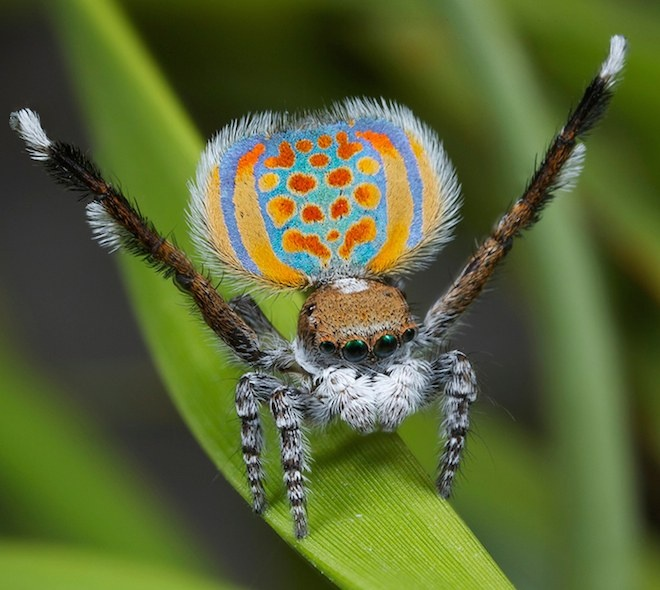
\includegraphics[width=0.3\textwidth]{RGB}
    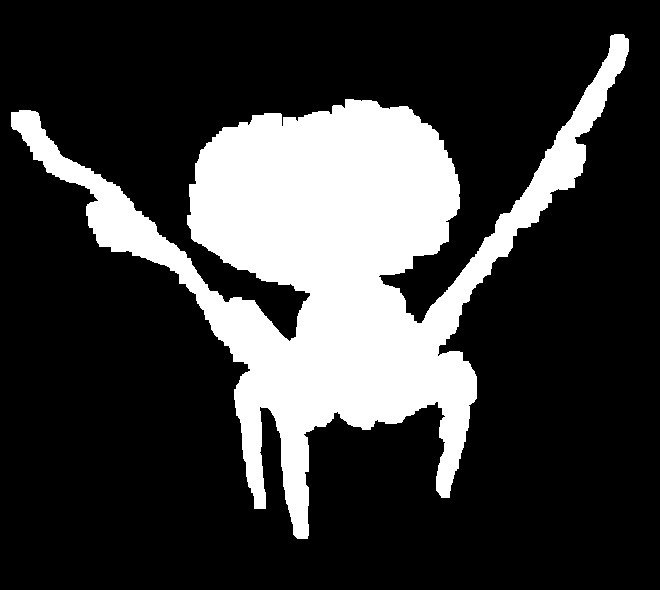
\includegraphics[width=0.3\textwidth]{mask}
    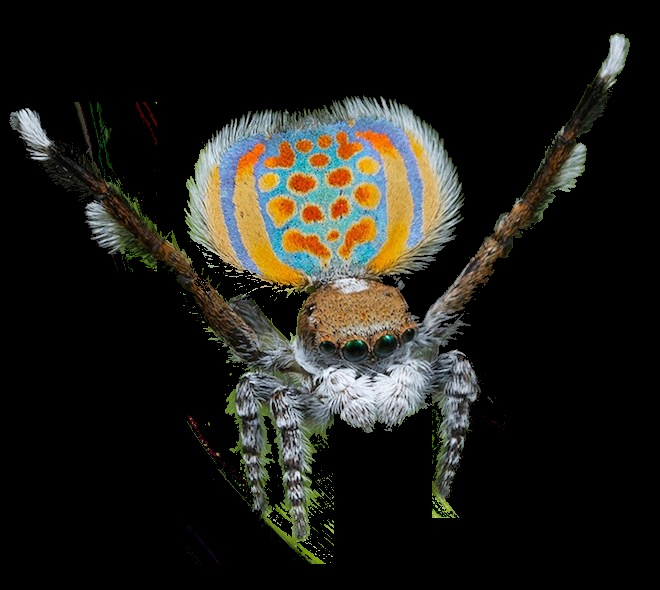
\includegraphics[width=0.3\textwidth]{masked}
    \caption{Da sinistra a destra: immagine originale, maschera binaria, risultato del masking}
    \label{fig:mask_example}
  \end{center}
\end{figure}

% TODO dire che ci sono vari tipi di masking?

% \clearpage
% \subsection {Traslazioni e Rotazioni}
% 
% Trasformazioni Affini
% % https://en.wikipedia.org/wiki/Digital_image_processing
% % https://en.wikipedia.org/wiki/Affine_transformation
% % https://en.wikipedia.org/wiki/Rotation
% 
% Come abbiamo accennato prima, le trasformazioni affini ci permettono di effettuare traslazioni e rotazioni alle immagini.
% 
% TODO
% 
% Con la matrice per il cambio di base
% % wrap affine e matrici di traslazione / rotazione
% % cfr cambio di base?
% \begin{figure}[ht] % TODO immagini
%   \begin{center}
%     \includegraphics[width=0.3\textwidth]{example-image}
%     \includegraphics[width=0.2\textwidth]{example-image}
%     \includegraphics[width=0.3\textwidth]{example-image}
%     \caption{TODO cambiare immagini}
%     \label{fig:traslation_example}
%   \end{center}
% \end{figure}

\clearpage
\subsection {Image Cropping and Resizing}
Quando si effettua un \textit{image cropping} si ritaglia una porzione dell'immagine, che viene chiamata ROI (\textit{Region Of Interest}), sulla quale vogliamo concentrare la nostra attenzione.
Dato che ogni immagine è rappresentata con una matrice, una ROI non sarà nient'altro che una matrice di dimensioni minori in cui sono stati copiati i valori dell'area interessata.
Una matrice di questo tipo viene anche chiamata \textit{view}.
% https://en.wikipedia.org/wiki/Cropping_(image)

Con l'\textit{image resizing} si aumentano (o diminuiscono) le dimensioni di un'immagine.
Nel primo caso, poiché si vuole aumentare il numero di pixel dell'immagine finale,bisognerà utilizzare tecniche di upsampling ed interpolare i dati a disposizione per generarne di nuovi che siano verosimili.

Uno fra gli algoritmi più semplici è Nearest-Neighbor Interpolation:
il pixel che deve essere aggiunto ottiene il valore del pixel a lui più vicino.
Un criterio di scelta dovrà essere definito nel caso in cui ci siano più pixel alla stessa distanza ma con valori differenti.
Un criterio possibile è quello di assegnare al nuovo pixel sempre il valore del pixel in alto a sinistra.
% https://en.wikipedia.org/wiki/Nearest-neighbor_interpolation
% https://docs.opencv.org/2.4/modules/imgproc/doc/geometric_transformations.html
% https://en.wikipedia.org/wiki/Image_scaling
% https://en.wikipedia.org/wiki/Scale_(ratio)

Una tecnica leggermente più complessa, ma che fornisce risultati soddisfacenti nella maggior parte delle occasioni, è l'interpolazione bilineare.
Con questa tecnica si effettuano, in cascata, due interpolazioni lineari, una orizzontale ed una verticale.
Con l'interpolazione bilineare i nuovi pixel si ottengono come media dei valori noti, pesata rispetto allo loro distanza dal pixel che si vuole colorare.
In questo modo si ottengono immagini con transazioni di colore più dolci.

% TODO
% Parentesi sulle formule?
% Linear Interpolation
% % https://en.wikipedia.org/wiki/Linear_interpolation
% per poi spiegare Bilinear Interpolation?
% % https://en.wikipedia.org/wiki/Bilinear_interpolation
% %https://theailearner.com/2018/12/29/image-processing-bilinear-interpolation/


Nel caso in cui si voglia ridurre le dimensioni dell'immagine si dovranno usare tecniche di \textit{downsampling} ed \textit{anti-aliasing}.
% https://en.wikipedia.org/wiki/Anti-aliasing_filter
Il downsampling permette di selezionare un numero limitato di pixel che poi verranno usati per colorare la matrice di dimensione ridotta.
Applicare soltanto questa tecnica può portare alla creazione di artefatti sintetici nell'immagine risultato.
Significa che l'immagine ridotta potrebbe contenere gruppi di pixel di colori sbagliati.
Sfruttando tecniche come l'anti-aliasing si può evitare, o quantomeno limitare, la creazione di tali artefatti.
Un \textit{low-pass filter} è un tipo di filtro che smorza tutti i valori al di sopra di una certa soglia, mentre lascia passare tutti i valori minori.
Nel campo del \textit{digital image processing} vengono utilizzati filtri di \textit{blur} applicati tramite convoluzione.
Il termine \textit{blur} o \textit{smooth} indicano applicare un effetto sfocato che tende a rendere più dolci le transizioni da un colore all'altro, andando quindi anche a ridurre valori troppo alti (o troppo bassi) avvicinandoli a valori più probabili.


\clearpage
\subsection {Histogram Equalization}
Questa tecnica permette di "aggiustare" il contrasto di un'immagine sfruttandone l'istogramma.
Il contrasto è definito come la differenza in intensità luminosa e colore che permette di distinguere gli oggetti.

In Figura~\ref{fig:hist_eq_example} sono stati riporta un'immagine a basso contrasto e l'immagine risultato dopo l'applicazione della \textit{histogram equalization}.
Sotto ogni immagine si possono osservare i relativi istogrammi: sull'asse delle $x$ abbiamo ogni possibile valore di un pixel, quindi da 0 a 255; sull'asse delle $y$ è riportato il numero di occorrenze di quel colore nell'immagine.
Notare che l'immagine in input deve essere in scala di grigi.

Vediamo ora come possiamo formulare matematicamente la costruzione dell'istogramma e la sua manipolazione.
Siano $X$ l'immagine di partenza ed $Y$ l'immagine risultato.
Facendo riferimento a quanto scritto nel documento l'istogramma può essere definito come:
\todo{TODO AGGIUNGERE REF A DOC}
\begin{equation*}
p_n = \frac{\text{\# di pixel di colore} \quad n}{\text{\# totale di pixel}} \quad \text{con} \quad n \in [0,255]
\end{equation*}
Poiché $p_n$ descrive la probabilità che un pixel, scelto a caso dall'immagine, abbia valore $n$, possiamo considerare $X$ una variabile casuale discreta in $[0,255]$.
Quindi $X$ avrà funzione di ripartizione, tracciata in nero nel grafico, pari ad:
\begin{equation*}
  F_X(x) = \sum_{n=0}^{x} p_n
\end{equation*}
Noi vorremmo che la differenza di colore tra i pixel fosse più netta, così da aumentare il contrasto dell'immagine.
Per raggiungere i nostri scopi possiamo ridistribuire equamente i valori di $X$ nell'intervallo dei valori possibili:
\begin{equation*}
  T(x) = \text{floor}(255 * F_X(x))
\end{equation*}
dove floor() arrotonda verso il basso all'intero più vicino.
In questo modo possiamo ottenere la variabile casuale trasformata $Y=T(X)$, ossia l'immagine equalizzata.
Sostanzialmente abbiamo ricolorato ogni pixel dell'immagine di partenza con colori più distanti tra loro.

\begin{figure}[ht] % TODO rifare grafici
  \begin{center}
    \begin{tabular}{cc}
      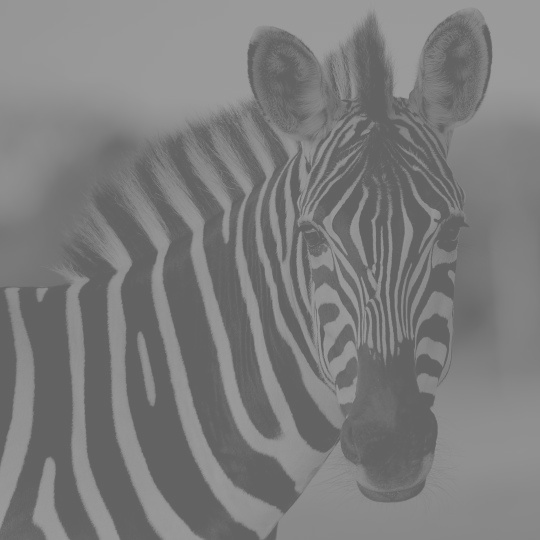
\includegraphics[width=0.3\textwidth]{GRAY_low_contrast} &
      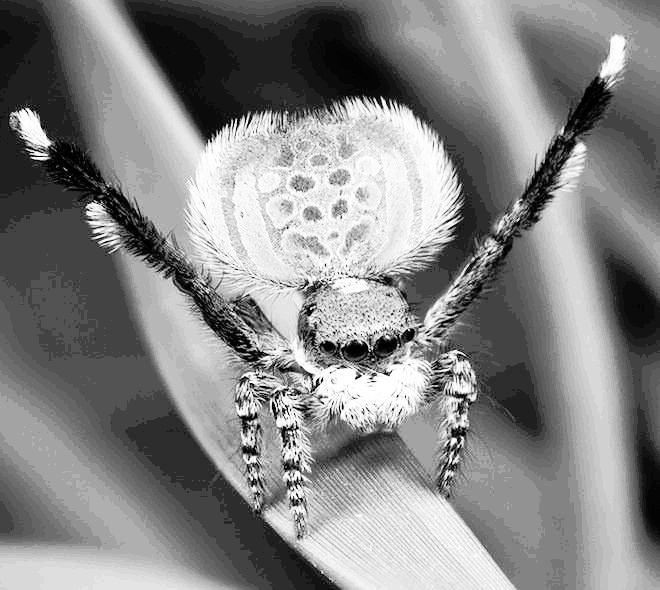
\includegraphics[width=0.3\textwidth]{eqHist_example} \\
      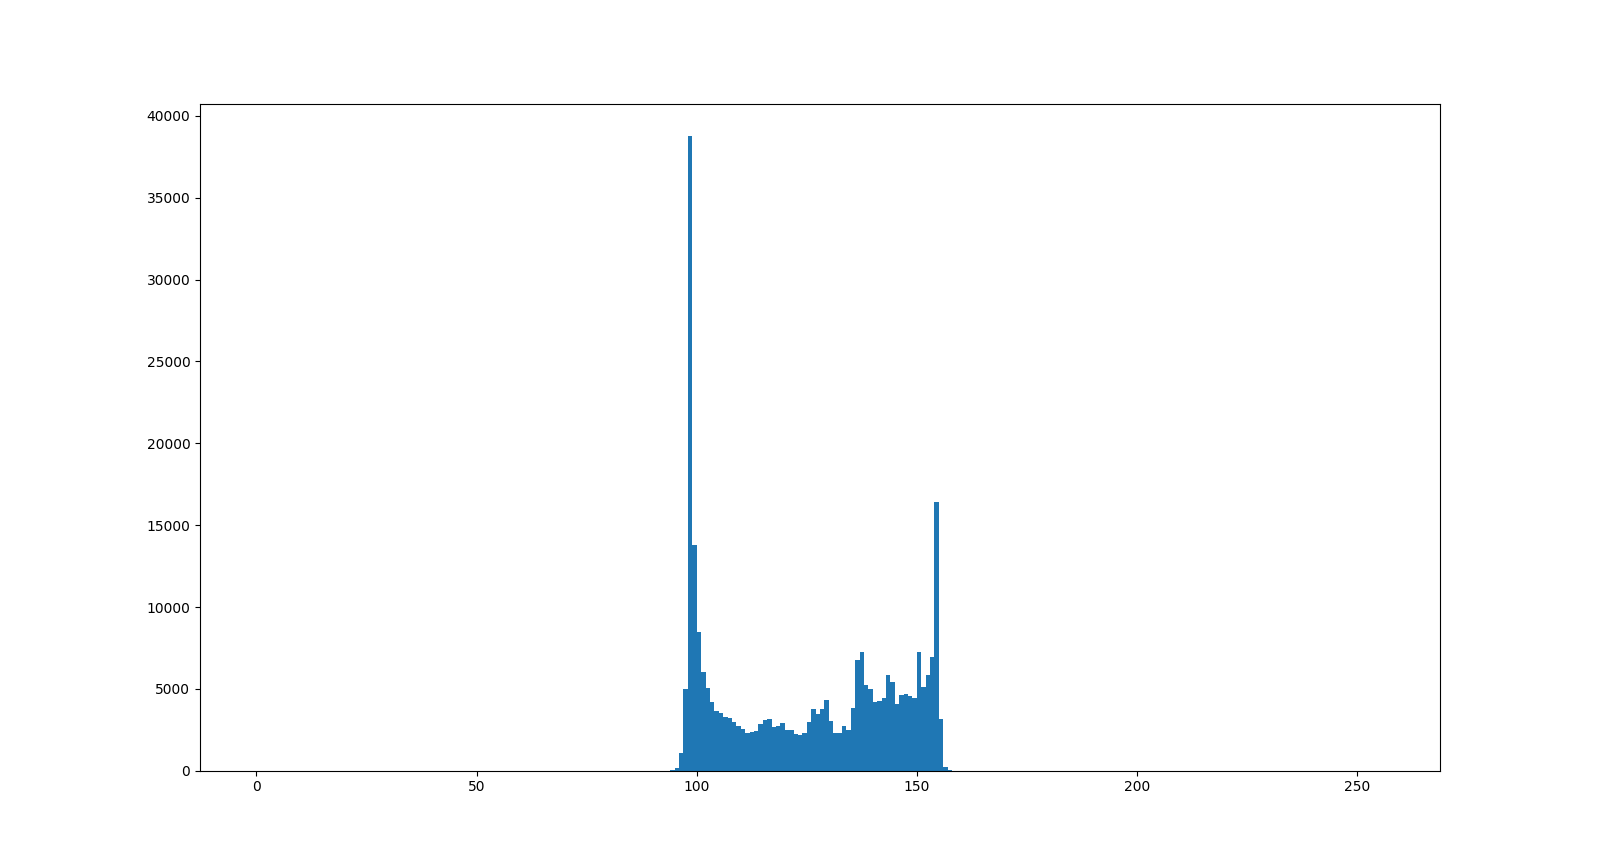
\includegraphics[width=0.3\textwidth]{pre_eq_hist} &
      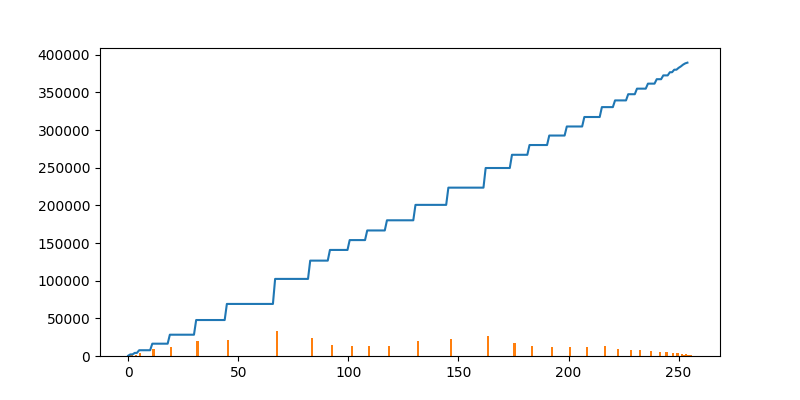
\includegraphics[width=0.3\textwidth]{post_eq_hist}
    \end{tabular}
    \caption{TODO rifare grafici}
    \label{fig:hist_eq_example}
  \end{center}
\end{figure}


% https://en.wikipedia.org/wiki/Histogram_equalization

\clearpage
\subsection {Gaussian Blur}
Conosciuto anche come \textit{Gaussian smoothing}, il \textit{Gaussian blur} permette di sfocare un immagine sfruttando una convoluzione con kernel gaussiano.
L'immagine così ottenuta risulta meno nitida, con meno dettagli e, quindi, con meno rumore.
L'obbiettivo principale di questa tecnica è mantenere soltanto l'informazione caratterizzante, rimuovendo quella non necessaria od anomala.
Si può dimostrare che il \textit{Gaussian blur} è un \textit{low-pass filter}.

Si ricorda che la funzione di Gauss ad un parametro è
\begin{equation*}
  G(x) = \frac{1}{\sqrt{2\pi\sigma^2}}
         \exp{\Bigl(- \frac{ x^2 }{ 2 \sigma^2 } \Bigr)} 
\end{equation*}
Si dimostra che la funzione di Gauss a due parametri equivale al prodotto di due funzioni come quella appena definita, in formule
\begin{equation}
  \begin{split}
    G(x,y) & = G(x)G(y) \\
           & = \frac{1}{2\pi\sigma^2}
               \exp{\Bigl(- \frac{ x^2 + y^2 }{ 2 \sigma^2 } \Bigr)} 
  \end{split}
\end{equation}
in cui $x$ ed $y$ sono le distanze dagli assi di riferimento, mentre $\sigma$ è la deviazione standard.
% In termini di calcolo computazionale ciò può essere sfruttato eseguendo due computazioni lineari,
% rispetto alle dimensioni dell'immagine e del kernel, %non corretto
% \todo{TODO correggere e dire meglio}
% anziché una quadratica.
% 
% $
% {\displaystyle O\left(w_{\text{kernel}}w_{\text{image}}h_{\text{image}}\right)+O\left(h_{\text{kernel}}w_{\text{image}}h_{\text{image}}\right)}
% $
% 
% $
% {\displaystyle O\left(w_{\text{kernel}}h_{\text{kernel}}w_{\text{image}}h_{\text{image}}\right)}
% $

La matrice sottostante rappresenta un filtro gaussiano quadrato di lato $7$ con $\sigma = 2$.

\begin{equation*} % TODO 
  \begin{bmatrix}
    0&0&0&0&0&0&0\\
    0&0&0&0&0&0&0\\
    0&0&0&0&0&0&0\\
    0&0&0&0&0&0&0\\
    0&0&0&0&0&0&0\\
    0&0&0&0&0&0&0\\
    0&0&0&0&0&0&0
  \end{bmatrix}
\end{equation*}
\todo[noline]{inserire valori}

Ricordiamo che durante una convoluzione si effettua la somma di prodotti elemento per elemento, ossia una media pesata in cui i pesi sono definiti nel kernel.
Dato che i valori al centro del filtro sono più grandi di quelli ai bordi, daremo maggior peso ai pixel nell'intorno dell'elemento su cui il kernel viene centrato.
Sappiamo che all'aumentare di $\sigma$ cresce il raggio alla base della campana di Gauss, questo significa che verrà data sempre più importanza ai pixel distanti.
Ciò farà risultare l'immagine in uscita molto più sfocata.

%\begin{figure}[ht] % TODO
%  \begin{center}
%    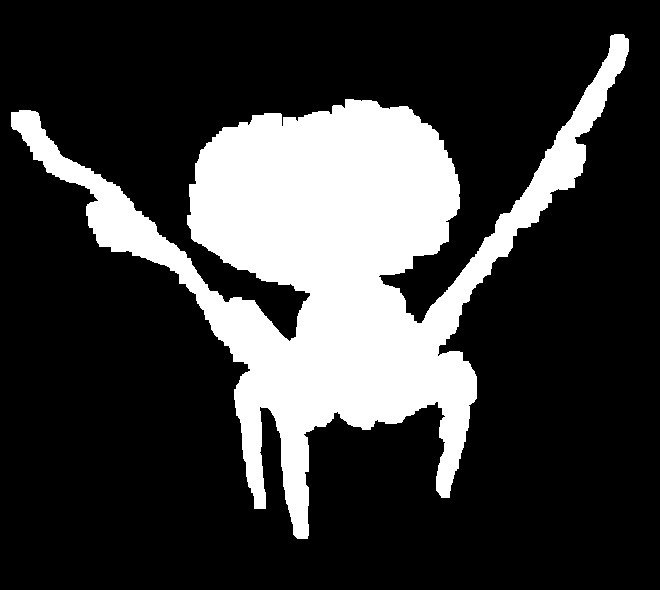
\includegraphics[width=0.3\textwidth]{mask} % plot 3d del kernel
%    \caption{TODO plot 3d del kernel}
%    \label{fig:gaussian_kernel}
%  \end{center}
%\end{figure}

In Figura~\ref{fig:gaussian_blur_example} è riportata un'immagine prima e dopo l'applicazione del filtro appena descritto, si nota come i dettagli più piccoli sono stati rimossi, mentre l'oggetto dell'immagine rimane distinguibile.

\begin{figure}[ht] % TODO
  \begin{center}
    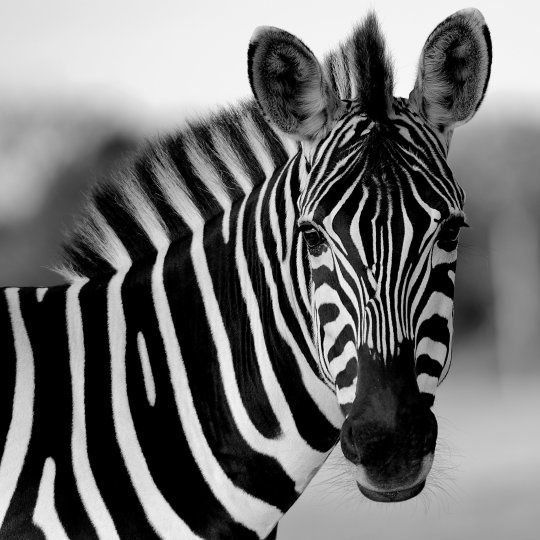
\includegraphics[width=0.4\textwidth]{GRAY}
    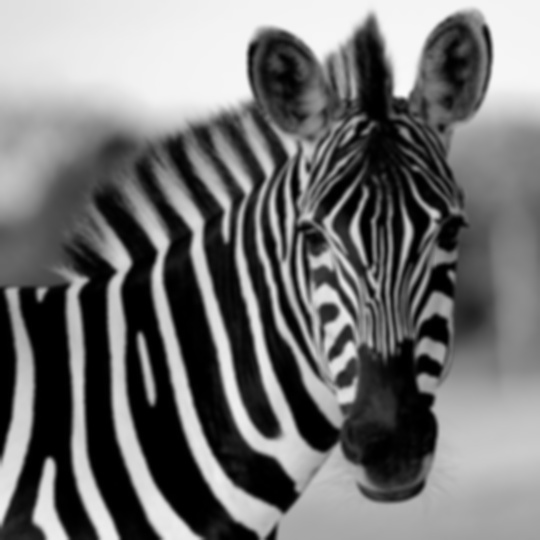
\includegraphics[width=0.4\textwidth]{gaussian_blur_example}
    \caption{TODO rifare caption}
    \label{fig:gaussian_blur_example}
  \end{center}
\end{figure}

Va fatta un'ultima considerazione: cosa succede se applico due volte lo stesso filtro?
Se si applica più volte uno stesso filtro gaussiano si ottiene lo stesso risultato che si otterrebbe dopo un'unica applicazione di un filtro 
\todo{TODO completare}

% https://en.wikipedia.org/wiki/Gaussian_blur

%\clearpage
%\subsection {Bilateral Filter}
%TODO
% https://en.wikipedia.org/wiki/Bilateral_filter
% https://docs.opencv.org/2.4/modules/imgproc/doc/filtering.html?highlight=bilateralfilter#bilateralfilter

% Capire formule in 
% http://homepages.inf.ed.ac.uk/rbf/CVonline/LOCAL_COPIES/MANDUCHI1/Bilateral_Filtering.htmlhttp://homepages.inf.ed.ac.uk/rbf/CVonline/LOCAL_COPIES/MANDUCHI1/Bilateral_Filtering.html


\clearpage
\subsection {Sobel Operator}
Prima di descrivere cosa sia il \textit{Sobel operator}, detto anche \textit{Sobel filter}, bisogna dare una definizione di gradiente.
% TODO formattare correttamente la citazione
Nel calcolo vettoriale, il gradiente è la generalizzazione della derivata.
La derivata di una funzione ad una variabile associa ad ogni punto uno scalare, mentre il gradiente di una funzione $f$ a più variabili associa ad ogni punto un vettore multidimensionale.
Quest'ultimo è composto dall'insieme delle derivate parziali di $f$ nel punto considerato.
Il gradiente rappresenta la pendenza della tangente al grafico della funzione in un punto.
La sua direzione indica il più grande incremento della funzione mentre la magnitudine è il tasso d'incremento.

Possiamo pensare un'immagine (in scala di grigi) come una funzione a due variabili che associa ad ogni punto $(x,y)$ un valore in $[0,255]$.
Il gradiente dell'immagine sarà composto da vettori direzionati in modo da uscire dalle zone scure ed entrare nelle zone più chiare (mantenendo la convenzione per cui a zero è associato il colore nero).
La magnitudine sarà tanto più grande quanto più grande il contrasto, quindi differenza di colore e luminosità.
%In Figura~\ref{fig:gradient} è presentato un esempio di gradiente di un'immagine.
%\begin{figure}[ht] % TODO
%  \begin{center}
%    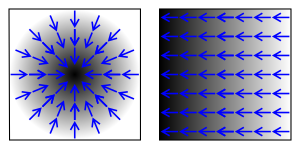
\includegraphics[width=0.2\textwidth]{gradient}
%    \caption{TODO occhio che qui black=high e white=low}
%    \label{fig:gradient}
%  \end{center}
%\end{figure}

Ora possiamo procedere con la descrizione del filtro di Sobel.
Il \textit{Sobel filter} viene utilizzato per creare immagini in cui si enfatizzano gli \textit{edge}.
Per \textit{edge} si intendono tutte quelle zone dell'immagine che corrispondono a bordi, margini o spigoli degli oggetti rappresentati nell'immagine.
Ciascuna di queste zone deve necessariamente essere associata almeno ad un cambio di colore oppure ad un cambio di luminosità, altrimenti l'oggetto in questione non sarebbe distinguibile dallo sfondo.
Quindi, osservando il gradiente dell'immagine, ad ogni \textit{edge} corrisponderà una serie di vettori con magnitudine più grande rispetto alle magnitudini dei vettori circostanti.
Lo scopo del \textit{Sobel operator} è generare una approssimazione del gradiente dell'immagine sfruttando due convoluzioni distinte con uno specifico kernel.
Nonostante il risultato sia abbastanza grossolano, la sua efficacia e rapidità lo rendono uno dei principali strumenti per la \textit{edge detection}, tecnica che esploreremo fra poco.

L'applicazione del filtro Sobel avviene come mostrato nelle due equazioni sottostanti, dove $*$ denota una convoluzione ed $I$ è un'immagine in scala di grigi.

\begin{equation} \label{eq:sobel_gx}
  G_x = 
  I
  *
  \begin{bmatrix}
    -1&0&1\\
    -2&0&2\\
    -1&0&1\\
  \end{bmatrix}
\end{equation}
\begin{equation} \label{eq:sobel_gy}
  G_y = 
  I
  *
  \begin{bmatrix}
    -1&-2&-1\\
    0&0&0\\
    1&2&1\\
  \end{bmatrix}
\end{equation}
\begin{equation} \label{eq:sobel_g}
  G = \sqrt{G_x^2 + G_y^2}
\end{equation}
%\begin{equation} \label{eq:sobel_angle}
%  \Theta = atan{\Bigl( \frac{G_y}{G_x} \Bigr)}
%\end{equation}
% TODO allineare le equazioni

La prima equazione fornisce un'approssimazione del gradiente rispetto all'asse $x$, mentre la seconda rispetto ad $y$.
La terza equazione, invece, combina le precedenti fornendoci informazione riguardo alla magnitudine del gradiente dell'immagine.

\todo{TODO aggiungere formula per angolo}

Ora verranno fatte delle considerazioni sul primo kernel ma, poiché il secondo è una semplice trasposta del primo, tali considerazioni sono, facendo riferimento all'asse delle $y$, valide anche per il filtro in equazione \ref{eq:sobel_gy}.
Il kernel nell'equazione~\ref{eq:sobel_gx} assegnerà valori in assoluto più grandi a pixel in una posizione di transizione di colore, rispetto a pixel posizionati in una zona con colorazione uniforme.
Prendiamo un pixel $p$ di colore bianco posizionato in una zona in cui tutti i pixel sono di colore bianco, si avrà che il kernel, pesando i pixel a destra allo stesso modo di quelli di sinistra ma con segno opposto, attribuisce un valore pari a $0$ a $p$.
Se $p$ fosse stato in una zona si transizione dal bianco al nero, avrebbe ottenuto un valore negativo molto grande:
tutti i valori nella prima colonna del filtro verrebbero moltiplicati per $255$ mentre tutti quelli dell'ultima colonna verrebbero annullati, essendo moltiplicati per $0$.


Nell'immagine sottostante viene mostrata l'applicazione dell'operatore Sobel prima rispetto ad $x$, poi rispetto ad $y$ ed infine il risultato della combinazione delle precedenti.

\begin{figure}[ht] % TODO
  \begin{center}
    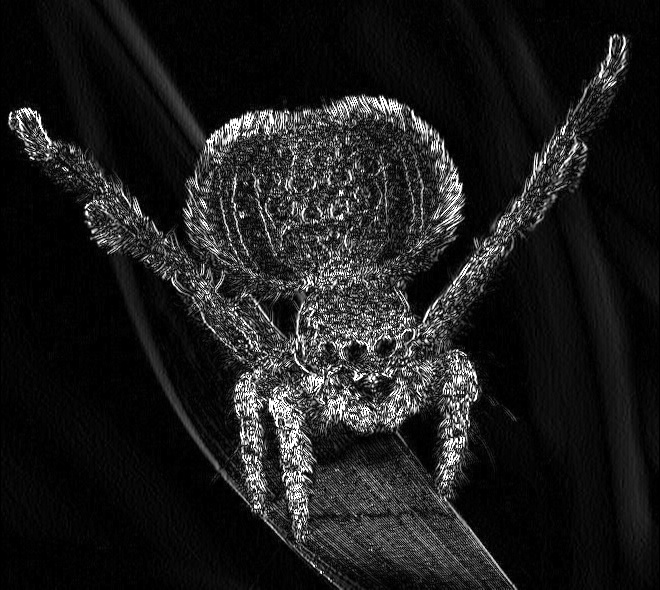
\includegraphics[width=0.3\textwidth]{gx}
    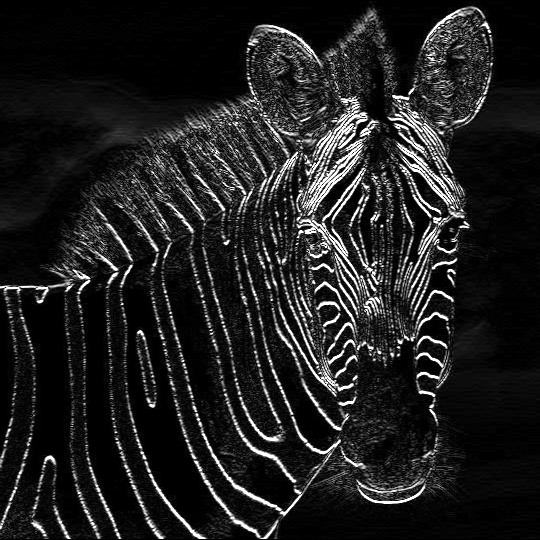
\includegraphics[width=0.3\textwidth]{gy}
    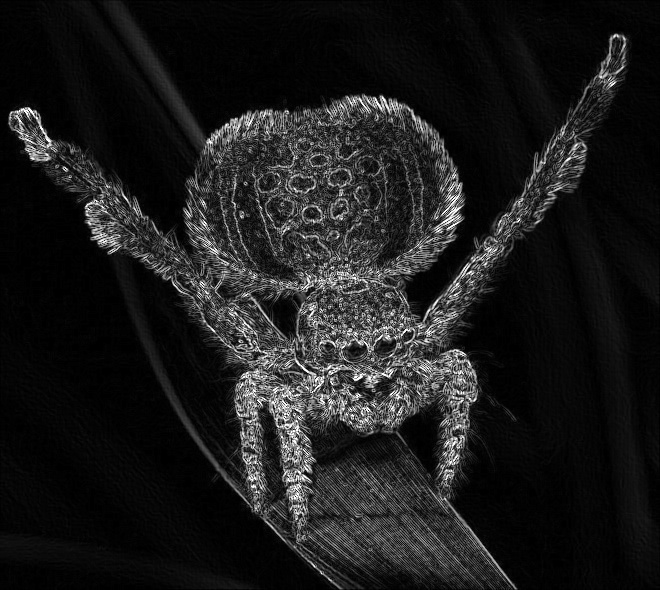
\includegraphics[width=0.3\textwidth]{g}
    \caption{TODO caption}
    \label{fig:sobel_example}
  \end{center}
\end{figure}
\todo{fare griglia più grande \\ aggiungere immagine originale}



% https://en.wikipedia.org/wiki/Sobel_operator
% https://en.wikipedia.org/wiki/Gradient

\clearpage
\subsection {Canny Edge Detector}
Composto da vari passaggi ed algoritmi, il \textit{Canny Edge Detector} permette di estrarre i principali \textit{edge} di un'immagine ottenendo risultati soddisfacenti ed adattabili alle necessità dell'utilizzatore.
Questo rilevatore viene sfruttato largamente come tecnica di \textit{feature extraction} perché permette di rimuovere molta informazione dall'immagine mantenendo solo quella strettamente necessaria.
Nell'ambito del \textit{edge detection} è bene che tutti gli \textit{edge} presenti nell'immagine vengano identificati correttamente, ma è altrettanto importante che non vengano generati falsi positivi, cioè che delle aree nel risultato presentino contorni che nell'immagine di partenza non esistevano.
Per questo motivo \textit{Canny edge detector} effettua molte operazioni di rimozione di falsi positivi ed allo stesso tempo tende ad evidenziare molto bene quelli che sembrano essere \textit{edge autentici}.
Ora verranno elencati in ordine i vari passaggi del rilevatore:
\begin{enumerate}
  \item Viene applicato un filtro gaussiano per effettuare uno \textit{smooth} all'immagine.
    Questo passaggio è fondamentale perché vengono rimossi valori anomali che, risultando come picchi positivi o negativi, potrebbero contribuire a generare falsi positivi.
    Inoltre rimuove può essere usato per rimuovere dettagli superflui.

  \item Utilizzando il \textit{Sobel operator} si ottiene la magnitudine dei gradienti dell'immagine, ossia tutti gli \textit{edge} candidati, che dovranno poi essere manipolati e selezionati.

  %\item Con il \textit{non-maximum suppression}  % TODO fare se c'e spazio

  \item Con una doppia sogliatura si ottengono due effetti:
    come prima cosa vengono rimossi tutti quegli edge con magnitudine troppo bassa, perché considerati rumore;
    successivamente gli edge sopravvissuti vengono classificati come forti e deboli, questa informazione verrà sfruttata nel prossimo passaggio.
    Effettuare una sogliatura significa semplicemente osservare ogni valore di un'immagine, nel nostro caso ogni pixel indica la magnitudine, e mapparlo ad un valore dato se soddisfa determinate condizioni.
    In questo passaggio sono presenti due soglie.
    La prima ci permette di annullare tutti gli edge con valori troppo piccoli.
    Con la seconda viene usata per etichettare i pixel superiori come \textit{strong edge}.
    Tutti i pixel intermedi vengono considerati \textit{weak edge}.

  \item A questo punto si procede con il rimuovere tutti gli edge deboli che non facciamo parte di edge forti.
    Significa che, per ogni pixel etichettato come \textit{weak edge}, vengono osservati gli otto pixel circostanti.
    Se nessuno di questi è uno \textit{strong edge} allora il pixel centrale viene annullato.
    % TODO cfr Connected Componets

\end{enumerate}
Va fatto notare che i valori delle due soglie devono essere trovati in modo empirico, a seconda del tipo d'immagine bisognerà impostare soglie più o meno grandi, ma anche più o meno distanti fra loro.

In Figura~\ref{fig:canny_example} è illustrata l'applicazione del \textit{Sobel operator}, notare come il risultato sia molto più pulito di quello illustro in Figura~\ref{fig:sobel_example}.
\begin{figure}[ht] % TODO
  \begin{center}
    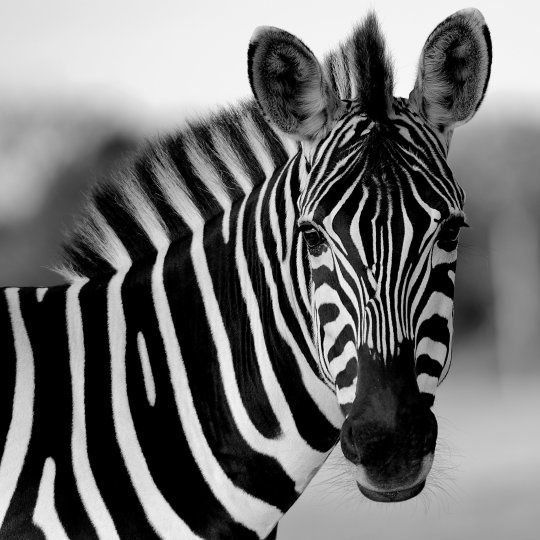
\includegraphics[width=0.4\textwidth]{GRAY}
    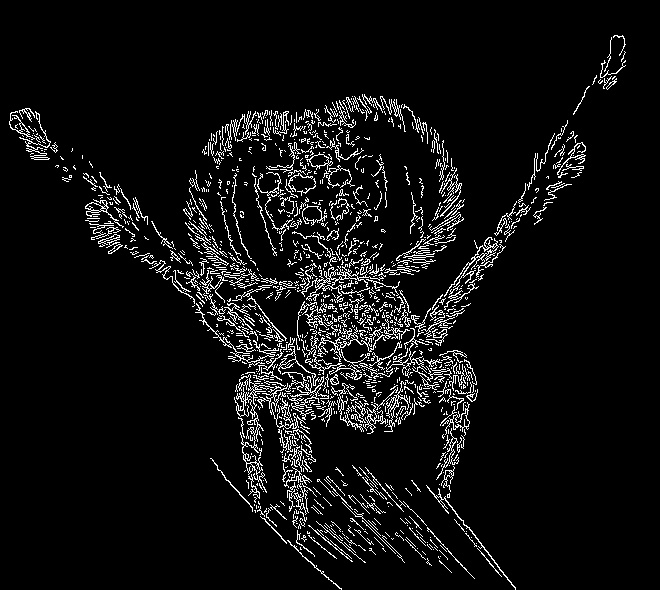
\includegraphics[width=0.4\textwidth]{canny_example}
    \caption{TODO }
    \label{fig:canny_example}
  \end{center}
\end{figure}


% https://en.wikipedia.org/wiki/Canny_edge_detector

\clearpage
\subsection {Hough Circle Transform}
Prima di poter spiegare questa tecnica si devono introdurre alcuni concetti come la \textit{Hough Line Transform}, lo \textit{Hough Parameter Space} e la parametrizzazione raggio-angolo di una retta.
Le trasformate di Hough sono largamente usate come metodi di \textit{feature extraction}, permettono di rilevare semplici figure come linee e cerchi.
Il loro obbiettivo è raggruppare correttamente un'insieme di pixel in modo che l'insieme raffiguri la forma che si vuole trovare.
Una delle problematiche principali è la possibilità che nell'immagine la forma da rilevare sia discontinua o deformata.

Esploriamo come il metodo di \textit{Hough Line Transform} permette di trovare una linea retta in un'immagine.
Definiamo tre punti $P_i=(x_i, x_i)$ con $i=1,2,3$ in modo che siano allineati, cioè che esista una retta a alla quale appartengano tutti.
Sappiamo che per ciascun punto ci sono infinite rette che soddisfano $y_i = m x_i + c$, ma che soltanto una di queste rette passa anche per gli altri due punti.
L'equazione appena descritta è in funzione di $m$ e $c$, riscrivendola come
\begin{equation} \label{eq:cm_lines}
  c = y_i - m x_i \quad con \quad i=1,2,3
\end{equation}
risulta più facile immaginarla (fissato un $i$) come una retta in uno spazio in cui $c$ è sull'asse delle ordinate e $m$ su quello delle ascisse.
Lo spazio appena descritto prende il nome di \textit{Hough Parameter Space}, in cui ogni punto $(m,c)$ descrive una retta nello spazio di partenza.
Nello \textit{Hough Parameter Space} le tre rette della formula \ref{eq:cm_lines} si devono necessariamente incontrarsi in esattamente un punto, sia $(m_0,c_0)$, perché sappiamo che deve esistere una coppia di parametri per cui la retta $y = m_0 x + c_0$, nello spazio originale, passa per tutti gli $P_i$.
L'idea alla base di \textit{Hough Line Transform} è quella di, definito un range di valori per $m$ e per $c$, trovare quello che soddisfa il maggior numero di equazioni.
In pratica ad ogni cella nello spazio $m$-$c$ viene associato un intero che indica quante delle rette di equazione~\ref{eq:cm_lines} ref passano per quella cella.

Ci si accorge facilmente che questo metodo non ci permette di rilevare rette parallele all'asse delle $y$, infatti bisognerebbe avere un parametro $m$ con valore che tende all'infinito.
Per risolvere questa problematica viene usata la parametrizzazione raggio-angolo.
Come si vede in figura~\ref{fig:hough_parametr_raggio-angolo}, ogni retta viene identificata da una coppia univoca $(r,\theta)$.
Nella coppia $r$ indica la distanza dall'origine al punto più vicino della retta, mentre $\theta$ indica l'angolo tra il segmento appena generato e l'asse delle $x$.
Ogni retta viene identificata dall'equazione:
\begin{equation} \label{eq:raggio_angolo_parametr}
  r = x_i cos \theta + y_i sin \theta \quad con \quad i=1,2,3
\end{equation}
ottenibile con semplici calcoli geometrici.
Questo significa che il fascio di rette nello spazio di partenza verrà descritto da curve nello \textit{Hough Parameter Space} $\theta$-$r$, come si vede in figura~\ref{fig:hough_parametr_raggio-angolo}.
Valutando le celle nello stesso modo di prima si ottiene la retta passante per i tre punti ma identificata dalla coppia $(r_0,\theta_0)$.

\begin{figure}[ht] % TODO
  \begin{center}
    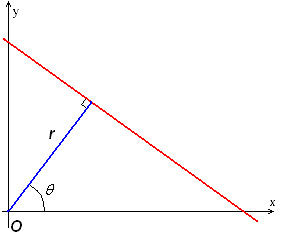
\includegraphics[width=0.3\textwidth]{raggio_angolo}
    \includegraphics[width=0.3\textwidth]{example-image}
    \caption{TODO }
    \label{fig:hough_parametr_raggio-angolo}
  \end{center}
\end{figure}


Vediamo ora come si può modificare la tecnica appena descritta per rilevare cerchi anziché linee rette.
L'idea principale ruota sempre attorno al concetto di voto di celle nello spazio di parametri.

In questo caso si sfrutta il fatto che, in una circonferenza $c$ di raggio $r$, ogni punto è equidistante dal centro.
Per ogni punto $P_i$ di $c$ può essere tracciata una circonferenza $c_i$ di centro $P_i$ e raggio $r$.
Sappiamo che tutte le circonferenze $c_i$ si incontrano in un unico punto, il centro di $c$, perché è l'unico equidistante da tutti i centri delle $c_i$.

Si ricorda che l'equazione di una circonferenza di centro $(a,b)$ e raggio $r$ è
\begin{equation} \label{eq:circonferenza}
  (x - a)^2 + (y - b)^2 = r^2
\end{equation}
Supponiamo di conoscere il raggio $r_0$ della circonferenza che vogliamo rilevare e di avere un insieme di punti $P_i$ che sappiamo appartenere alla circonferenza.
Lo spazio dei parametri $a$-$b$ ci permette di creare le circonferenze centrate nei $P_i$ e di assegnare un punteggio alto alla cella in $(a_0,b_0)$ perché votata da molte circonferenze.

Se anche il raggio fosse incognito allora lo \textit{Hough Parameter Space} avrebbe tre dimensioni ed ogni punto sarebbe una tripla $(a,b,r)$ appartenente alla superficie di un cono.
In figura~\ref{fig:hough_parametr_3d} è illustrata una rappresentazione di questo spazio.

Le implementazioni della \textit{Hough Circle Transform} sfruttano una matrice di supporto, chiamata accumulatore, che corrisponde allo spazio dei parametri di Hough.
Ciascun elemento è un intero con valore iniziale zero, che verrà incrementato di uno per ogni linea passante.

\begin{figure}[ht] % TODO
  \begin{center}
    \includegraphics[width=0.3\textwidth]{example-image}
    \includegraphics[width=0.3\textwidth]{example-image}
    \caption{TODO }
    \label{fig:hough_parametr_3d}
  \end{center}
\end{figure}

% TODO commento sulla implementazione 
% - immagine deve essere canny edge
% - threshold per fare pochi FP
% - min e max radius per restringere la ricerca


% Risorse
% https://docs.opencv.org/2.4/doc/tutorials/imgproc/imgtrans/hough_circle/hough_circle.html
% https://en.wikipedia.org/wiki/Hough_transform
% https://en.wikipedia.org/wiki/Circle_Hough_Transform

\clearpage
\subsection {Applicazione degli algoritmi descritti}
Si fa notare che prima di ottenere immagini come quella illustrata in Figura~\ref{fig:prima_dopo_prep} e soprattutto prima di essere sicuri che questo è il tipo di immagine migliore per i nostri scopi, sono stati necessari numerosi esperimenti e tentativi.
In particolar modo è stato importante capire che tipo di informazione potesse essere gestita interamente dalla rete neurale e quale invece dovesse essere rimossa o modificata.
Lo scopo del nostro \textit{pre-processing} è quello di fornire un'immagine contenente solo l'informazione necessaria e sufficiente per poter discriminare un pezzo conforme da uno scarto.

Nonostante in questa sezione vengano mostrate solo immagini di carcasse conformi, il processo iterativo appena descritto è stato eseguito confrontando costantemente immagini conformi e scarto.
Immagini scarto verranno mostrate nella prossima sezione, interamente dedicata a loro.

% https://tex.stackexchange.com/questions/343605/latex-code-for-subcaption-of-image
\begin{figure}[ht] % TODO
  \begin{center}
    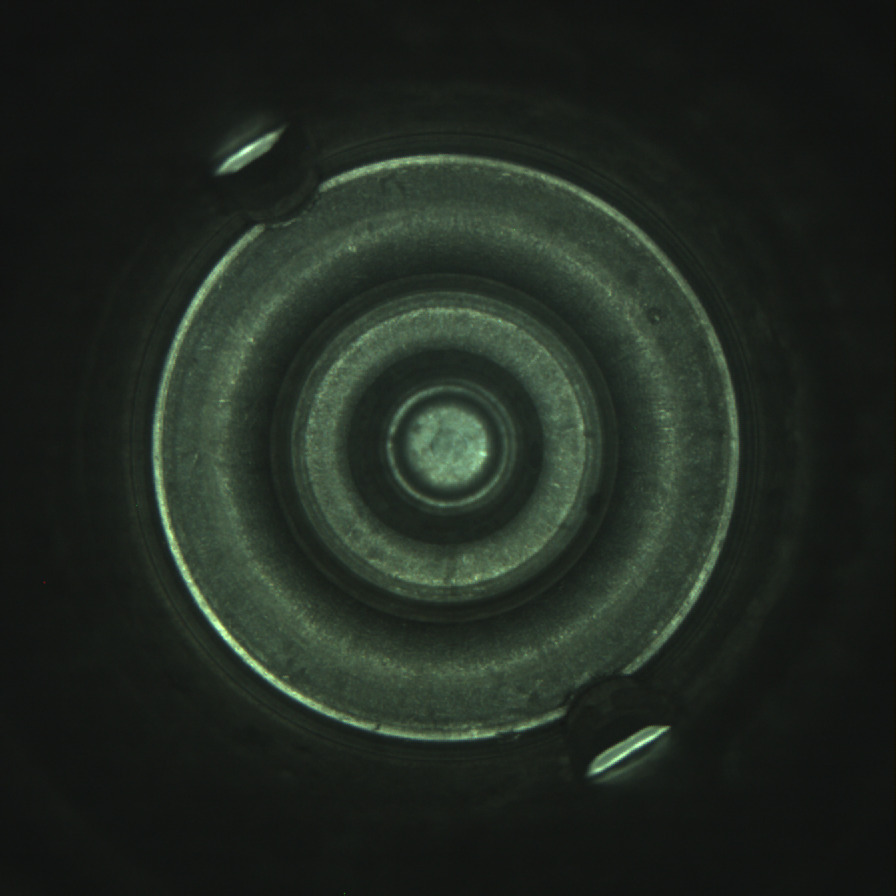
\includegraphics[width=0.5\textwidth]{128___1362_1_1_1_OnLineAnalysis}
    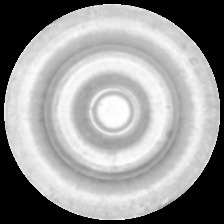
\includegraphics[width=0.35\textwidth]{128___1362_1_1_1_OnLineAnalysis_prep}
    \caption{TODO }
    \label{fig:prima_dopo_prep}
  \end{center}
\end{figure}

\clearpage
Ora verrà illustrato l'ordine in cui sono stati applica gli algoritmi descritti precedentemente e i principali motivi per cui sono stati scelti.

\subsubsection{1 Centramento con Hough Circle Transform}
Sappiamo che le immagini del dataset non sono perfettamente centrate, per questo motivo si è deciso di utilizzare la tecnica della \textit{Hough Circle Transform} per ottenere un'approssimazione del centro della carcassa.
Avendo le coordinate di quest'ultimo si riallineare il pezzo con il centro dell'immagine.
% TODO si può specificare che l'immagine deve essere
% - To Grayscale
% - Equalization Histogram
% - ottenere i cerchi con Hough Circle
% - media tra centri
% - trasformazione affine
% - l'immagine uscita è ancora a colori

Nella Figura~\ref{fig:centramento} sono illustrati, a sinistra, il cerchio rilevato, mentre sulla destra l'immagine prima e dopo il centramento.
\begin{figure}[ht] % TODO
  \begin{center}
    \includegraphics[width=0.3\textwidth]{example-image}
    \includegraphics[width=0.3\textwidth]{example-image}
    \includegraphics[width=0.3\textwidth]{example-image}
    \caption{TODO }
    \label{fig:centramento}
  \end{center}
\end{figure}

\subsubsection{2 Equalizzazione}
Per gestire la variazione di luminosità tra immagini si utilizza \textit{equalization histogram}.
In questo modo le immagini in bianco e nero delle carcasse risultano molto più simili tra di loro e si vanno a mitigare i fastidiosi effetti di sovra illuminazione.

D'ora in poi verranno manipolate immagini in scala di grigi.
Questa scelta, validata dagli esperimenti, nasce principalmente dalla prossima considerazione.
Le immagini sono in falsi colori, manterremmo informazione non reale ma soprattutto richiederemmo alla nostra rete neurale uno sforzo molto maggiore.
La rete, infatti, dovrebbe imparare a gestire non solo le forme geometriche del pezzo ma anche le sue colorazioni.

Nella Figura~\ref{fig:equalizzazione} sono illustrate due carcasse conformi con luminosità differenti, affiancate dalla loro trasformazione.
% TODO mostrare l'immagine gray scale prima e dopo
\begin{figure}[ht] % TODO
  \begin{center}
    \begin{tabular}{cc}
      \includegraphics[width=0.3\textwidth]{example-image} &
      \includegraphics[width=0.3\textwidth]{example-image} \\
      \includegraphics[width=0.3\textwidth]{example-image} &
      \includegraphics[width=0.3\textwidth]{example-image}
    \end{tabular}
    \caption{TODO}
    \label{fig:equalizzazione}
  \end{center}
\end{figure}

% TODO si può specificare che l'immagine deve essere
% - To Grayscale
% - Equalization Histogram

\subsubsection{3 Smooth dell'immagine}
Utilizzando un filtro gaussiano è stato rimosso il rumore principale, ossi quello dovuto a graffi ed effetto "sale e pepe".
È stato fondamentale definire il filtro in modo che non fosse troppo aggressivo altrimenti si sarebbe rischiato di perdere l'informazione della colla.

In Figura~\ref{fig:smooth} si mostra l'effetto dell'applicazione del kernel.
% TODO mostrare anche cosa succede se si esagera col filtro?
\begin{figure}[ht] % TODO
  \begin{center}
    \includegraphics[width=0.3\textwidth]{example-image}
    \includegraphics[width=0.3\textwidth]{example-image}
    \caption{TODO}
    \label{fig:smooth}
  \end{center}
\end{figure}

\subsubsection{4 Mascheramento}
L'area che nell'immagine corrisponde alla parete verticale della carcassa, ed in particolar modo alle due balze, deve essere rimossa.
Come abbiamo già sottolineato precedentemente la posizione delle balze non è correlata con la presenza della colla.
Mentre si suppone che la colla non si presenti soltanto sulla parete verticale, ma che coli almeno fino a raggiungere il gradino più ampio.

Nella Figura~\ref{fig:mask} è illustrato un conforme prima e dopo il mascheramento.
Fra le due immagini si presenta la maschera utilizzata.

\begin{figure}[ht] % TODO
  \begin{center}
    \includegraphics[width=0.3\textwidth]{example-image}
    \includegraphics[width=0.3\textwidth]{example-image}
    \includegraphics[width=0.3\textwidth]{example-image}
    \caption{TODO}
    \label{fig:mask}
  \end{center}
\end{figure}

\subsubsection{5 Crop}
A questo punto l'immagine contiene una grande porzione di pixel di colore nero, a causa del mascheramento.
Possiamo effettuare in operazione di \textit{crop} sapendo che il pezzo è centrato nell'immagine e conoscendo il raggio dell'area nera.
Osservando Figura~\ref{fig:crop} ci si accorge che dopo il ritaglio l'immagine trasporta, in proporzione, molta più informazione.

\begin{figure}[ht] % TODO
  \begin{center}
    \includegraphics[width=0.3\textwidth]{example-image}
    \includegraphics[width=0.3\textwidth]{example-image}
    \caption{TODO}
    \label{fig:crop}
  \end{center}
\end{figure}

\subsubsection{6 Resizing}
Come ultima cosa viene effettuato un resizing dell'immagine.
Ogni elemento del dataset ha originariamente una dimensione di $896$x$896$ pixel, dopo le trasformazioni effettuate abbiamo un'immagine di dimensione circa $580$x$580$.
Si fa notare che molte architetture di reti neurali accettano immagini di dimensione $224$x$224$.
Abbiamo verificato se questa dimensione fosse accettabile anche nella nostra applicazione: risulta che mantenere l'immagine ad una dimensione maggiore non comporta alcun vantaggio, mentre ridurla al di sotto dei $200$ pixel di lato rende la classificazione difficile anche per un essere umano.

% $896$x$896$
% $580$x$580$ % TODO verificare dimensione effettiva
% $224$x$224$

\section {Data Augmentation}
% Com'è stato sfruttato la Data Aug
% Colle sintetiche
Due metodi principali:
 - rotazione
 - generazione degli scarti sintetici

\subsection {Generazione Scarti Sintetici}


Scarti Sintetici
 I ritagli non sono stati semplicemente incollati sui conformi:

 la luminosità della colla è stata modificata per avvicinarsi a quella del pezzo conforme;
 dopo aver aggiunto la colla è stato praticato uno smooth lungo il contorno, per evitare che ci fosse una transizione netta fra sofndo ed inizio bordo della colla.







































% TODO in caso sarebe un Chapter a sé
%\section {La strada proposta}
% Simile a quanto detto in considerazioni_pixelwise_diff
%Mostrare qual'è l'obbiettivo che si vuole raggiungere con gli AE
%Spiegare che sono elastici e facili da allenare
%Il dataset non richiede dispendioso labeling


%!TEX TS-program = pdflatex
%!TEX root = tesi.tex
%!TEX encoding = UTF-8 Unicode

\chapter{Gli Autoencoder}

%%%%%%%%%%%%%%%%%%%%%%%%%%%%%%%%%%%%%%%%%%%%%%%%%%%%%%%%%%%%%%%%%%%%%%%%%%%%%%%%
% ROBE GENERALI DA FARE
% commento sotto dirlo ora o quando faccio la diff la prima volta nella sezione degli AE? Oppure quando creo gli scarti sintetici?
% Come ultima cosa accennare al fatto che gli scarti presentano anelli di colorazione differente e che questo sarà un grave problema in fase di valutazione dei risultati
% Specificare che NON è una proprietà "corretta" ma che dipende dal modo in cui sono state raccolte le immagini
% Che gli scarti on-line saranno uguali a Conforme+Colla
%%%%%%%%%%%%%%%%%%%%%%%%%%%%%%%%%%%%%%%%%%%%%%%%%%%%%%%%%%%%%%%%%%%%%%%%%%%%%%%%
%%%%%%%%%%%%%%%%%%%%%%%%%%%%%%%%%%%%%%%%%%%%%%%%%%%%%%%%%%%%%%%%%%%%%%%%%%%%%%%%
%%%%%%%%%%%%%%%%%%%%%%%%%%%%%%%%%%%%%%%%%%%%%%%%%%%%%%%%%%%%%%%%%%%%%%%%%%%%%%%%
% ATTENZIONE QUESTA E' LA CONVOLUZIONE IN UN LAYER CONVOLUTIVO
% INVECE IN QEUSTA SEZIONE QUA BISOGNA CENTRARE I KERNEL SU OGNI VALORE E 
% SOSTITUIRLO IN OUTPUT CON IL VALORE OTTENUTO
% NELLA SEZIONE SUGLI AE SPIEGO CHE D'ORA IN POI LE CONVOLUZIONI SONO DA INTENDERE 
% DIVERSAMENTE CIOE' CON QUALITA' DI FEATURE EXTRACTION (NOTA SUL PADDING CHE FA TORNARE LE CONV DEL AE COME QUELLE DA DESCRIVERE QUA)
% 
% Nell'ambito del \textit{Image Processing} con convoluzione si intende l'operazione che permette di effettuare, per ogni pixel dell'immagine, una somma pesata tra il pixel e gli elementi a lui vicini.
% I pesi sono definiti in una matrice, detta \textit{kernel} o filtro, di dimensioni non superiori a quelle dell'immagine di partenza.
% Solitamente i kernel hanno dimensione $3x3$ o $5x5$.
% Sfrutteremo ora un esempio per spiegare come viene effettuata una convoluzione, più avanti, quando parleremo del filtro Sobel, verrà illustrato lo pseudocodice che ne formalizza i passaggi.
% In Figura~\ref{fig:conv_example} sono illustrate, da sinistra a destra: l'immagine di partenza $I$, il filtro $K$ e l'immagine risultato $Y$.
% Il simbolo $*$ denota l'operazione di convoluzione e non è da confondere con nessun tipo di prodotto.
% Effettueremo una convoluzione da sinistra a destra e dall'alto verso il basso, ma si fa presente che l'ordine d'esecuzione non modifica il risultato.
% \begin{itemize}
%   \item Il primo passo è posizionare una copia di $K$ sopra ad $I$ in modo che l'angolo in alto a sinistra del kernel combaci con quello in alto a sinistra dell'immagine.
%   \item Ora possiamo moltiplicare ogni elemento di $I$ con il rispettivo elemento di $K$.
%     I valori così ottenuti dovranno essere sommati tra di loro.
%     Effettuando i conti si osserva che il risultato combacia con il valore in alto a sinistra dell'immagine risultato.
%   \item Il prossimo passo consiste nel far traslare il kernel di una cella a sinistra, calcolare la somma di prodotti rispetto ai nuovi valori ed infine salvare il risultato in $Y$ una cella a destra rispetto a prima.
%   \item Si prosegue in questo modo fino a che l'ultima colonna di $K$ non combacia con l'ultima colonna di $I$, questo coincide con il riempimento della prima riga in $Y$.
%   \item Ora bisogna posizionare $K$ in modo che l'elemento nell'angolo superiore sinistro sia sopra all'elemento in $I$ sulla prima colonna della seconda riga.
%     Si effettuano prodotti e somme, salvando il risultato nella prima cella libera della seconda riga in $Y$.
%   \item Si procede in questo modo finché non si raggiunge l'ultimo elemento dell''immagine di partenza.
% \end{itemize}
% 
% L'algoritmo può essere facilmente espresso tramite due cicli $for$ facendo attenzione a posizionare il kernel sempre entro i limiti dell'immagine di partenza.
% 
% \begin{figure}[ht]
%   \begin{center}
%     \includegraphics[width=0.6\textwidth]{esempio_convoluzione}
%     \caption{TODO Immagine da rifare}
%     \label{fig:conv_example}
%   \end{center}
% \end{figure}
%
% % TODO parentesi su il caso a colori?
% %%%%%%%%%%%%%%%%%%%%%%%%%%%%%%%%%%%%%%%%%%%%%%%%%%%%%%%%%%%%%%%%%%%%%%%%%%%%%%%%


\section{La Struttura di un Autoencoder}
% Struttura di un AE e differenze principali con CONV NN
Un Autoencoder (AE) è un particolare tipo di rete neurale il cui scopo è codificare efficacemente l'informazione fornita in input con modalità unsupervised.
Gli Autoencoder sono stati largamente utilizzati come tecniche per la dimensionality reduction, dimostrando capacità paragonabili a quelle di algoritmi come PCA o t-sne.
Un Autoencoder è formato da due componenti principali:
\begin{itemize}
    \item l'encoder, ottimizzato per generare una version compressa del dato;
    \item il decoder, ottimizzato per ricostruire l'informazione originale a partire dalla versione compressa.
\end{itemize}
Durante l'allenamento (training) la rete cerca di fornire un output il più simile possibile all'input ricevuto.
Potrebbe sembrare che l'obiettivo % TODO
dell'Autoencoder sia simulare la funzione identità, cioè quella funzione che fornisce in output esattamente l'input ricevuto.
In realtà all'interno della rete accade molto di più.
Prendiamo in esempio il più semplice degli AE: due layer fully-connected messi in sequenza.
Sappiamo che il numero di feature \footnote{TODO spiegare cosa si intende per feature} in ingresso nel primo layer deve combaciare con il numero di feature in uscita, altrimenti non potremmo confrontare l'input con la ricostruzione generata dalla rete.
Se si immaginano le feature in ingresso come dei punti, vettori, in un spazio n-dimensionale, con n pari al numero delle feature fornite, il compito dell'Autoencoder è generare dei punti che siano molto vicini ai punti osservati.
In altre parole si vuole che l'Autoencoder catturi la distribuzione probabilistica dei vettori forniti.
Stabilito, quindi, che la rete riceve e restituisce vettori di dimensionalità n si può definire la dimensionalità dello spazio latente, cioè di quello spazio di dimensione m, con $m < n$, in cui tutti i  vettori in input vengono mappati durante l'encoding.
Viene chiamato spazio latente perché non è conosciuto a priori.
Infatti sarà proprio la rete stessa, durante il training, a trovarlo, selezionandolo tra gli infiniti spazi m-dimensionali.
La dimensione dello spazio latente deve essere sufficientemente grande da permettere di mantenere le informazioni che caratterizzano l'input, ed allo stesso tempo sufficientemente piccolo così da rimuovere eventuale rumore o dati superflui.
Poco fa abbiamo definito due layer fully-connected, specificando soltanto le dimensioni in input del primo e le dimensioni in output del secondo.
Ora sappiamo che le feature in uscita dal primo layer dovranno essere accettate, in entrata, dal secondo.
Sappiamo anche che la dimensione della feature, in quanto vettore dello spazio latente, dovrà essere pari ad $m$.
La rete appena definita e raffigurata in %TODO figura
con la tipica forma a clessidra.
La parte più stretta di un Autoencoder è detta bottleneck (in italiano: collo di bottiglia) e corrisponde con la compressione massima del dato.

%TODO aggiungere formulazione matematica

\subsection{Variazioni dell'architettura}
Breve descrizione diconvAE stacked SAE DAE VAE


\subsection{Applicazioni principali}

La capacità degli Autoencoder di ricostruire l'input, quindi di mantenerne la struttura, privandolo di eventuale rumore o addirittura rimpiazzando il rumore con valori verosimili, si è rilevata utile in molti campi.

% TODO link ad anomaly detection
Quando il rumore incide notevolmente

% TODO link a paper image restoration
In questo paper si usano gli AE per colorare immagini un bg

Anche in questo documento la rimozione del rumore sarà un tema centrale, l'applicazione nel nostro caso verrà analizzato nel dettaglio nei prossimi capitoli.









\section {Convoluzioni e Convoluzioni Trasposte}
% Spiegazione dettagliata dei Conv Layers e dei Conv Transpose Layers
\section {Spazi Latenti}
% Sfruttabilità degli spazi latenti ed esempi di applicazioni



%!TEX TS-program = pdflatex
%!TEX root = tesi.tex
%!TEX encoding = UTF-8 Unicode

\chapter{Valutazione Sperimentale}


%!TEX TS-program = pdflatex
%!TEX root = tesi.tex
%!TEX encoding = UTF-8 Unicode

\chapter{Risultati Ottenuti}
\todo[inline]{sommario capitolo}
% descrizione architettura migliore e a chi ci siamo ispirati N.R.
\todo[inline]
{
  Preambolo sulla accuratezza dei modelli creati
  Problema dell'AE perché non fornisce accuratezza, come parametro di valutazione si è utilizzata la loss
  La loss non poteva essere usata come discrtiminatoe perché troppo poco sensibile all'errore di presenza-nonpreseena della colla
  Un altro criterio di valutazione era una verifica a mano della qualità della differenza conforme in out

  Descrivere architettura migliore
  Descrivere post-processing a valle
}

\clearpage
\section{Il nostro obbiettivo TODO}
In figura~\ref{fig:obbiettivo_in_out_diff} sono riportate tre immagini per chiarire in che modo gli \textit{autoencoder} sono stati sfruttati per classificare Conformi e Scarti.
La figura~\ref{fig:obbiettivo_in} illustra uno Scarto.
L'immagine riportata in figura~\ref{fig:obbiettivo_out} è quella che si vorrebbe ottenere dall'AE a partire dallo Scarto appena illustrato.
Notare come si vorrebbe che il pezzo fosse riprodotto il più fedelmente possibile, ma che l'informazione della colla venisse rimossa.
In questo modo sarebbe possibile effettuare una differenza $pixel$ per $pixel$ tra immagine in ingresso ed immagine in uscita (detta anche ricostruita) ottenendo così un risultato simile a quello in figura~\ref{fig:obbiettivo_diff}.

Nel caso migliore possibile la classificazione verrebbe effettuata verificando se nell'immagine differenza tutti i valori sono zero.
Ossia l'immagine in ingresso appartiene alla classe Conforme ed è stata ricostruito alla perfezione.
Dato che ci si aspetta che l'autoencoder non ricostruisca la colla nell'immagine in uscita, nell'immagine differenza ci sarà un'area di pixel con valori in assoluto maggiori di zero.

Non possiamo aspettarci che l'autoencoder abbia una precisione così alta, ingatti è molto più probaile che l''immaine ricostruita sia soltatnot un''approssimzione dell'immagine in ingresso. \todo{fix here}
Si ricorda che molto probabilemte l'AE rimuoverà tutte quelle caratteristiche particolari di un pezzo (graffi, macchie, \dots )



Quindi la classificazione è divisa in due parti: prima l'immagine viene passata dell'autoencoder; poi viene effettuato del post-processing.

\begin{figure}[ht] % TODO
  \begin{center}
    \begin{tabular}{ccc}

      \begin{subfigure}{.3\linewidth}
        \centering\includegraphics[width=\textwidth]{example-image}
        \caption{Immagine in ingresso}
        \label{fig:obbiettivo_in}
      \end{subfigure} &

      \begin{subfigure}{.3\linewidth}
        \centering\includegraphics[width=\textwidth]{example-image}
        \caption{Immagine ricostruita}
        \label{fig:obbiettivo_out}
      \end{subfigure} &

      \begin{subfigure}{.3\linewidth}
        \centering\includegraphics[width=\textwidth]{example-image}
        \caption{Immagine differenza}
        \label{fig:obbiettivo_diff}
      \end{subfigure}

    \end{tabular}
    \caption{TODO in out diff}
    \label{fig:obbiettivo_in_out_diff}
  \end{center}
\end{figure}



\clearpage
\section{Metriche di valutazione}




\clearpage
\section{Architettura dell'autoencoder}

\begin{figure}[ht]
  \begin{center}
    \includegraphics[width=\textwidth]{example-image}
    \caption{TODO architettura della rete}
    \label{fig:ae16_arch}
  \end{center}
\end{figure}

\begin{figure}[ht]
  \begin{center}
    \includegraphics[width=0.8\textwidth]{loss_plot}
    \caption{TODO plot della loss}
    \label{fig:loss_plot}
  \end{center}
\end{figure}

\clearpage
\section{Post-Processing}


%!TEX TS-program = pdflatex
%!TEX root = tesi.tex
%!TEX encoding = UTF-8 Unicode

\chapter{Metodi Alternativi}

% metrica di valutazione con loss

% ResNet + OCSVM 2 pagine
% Symmetric Skip e come ricrea la colla 1 pagina
% AE solo fully connected - interessante vedere come l'immagine venisse imparata a pixel - 1pagina + qualche immagine?
% AE solo convolutivi - incapacità di astrazione - mezza pagina


% tecniche classiche come quella roba della texture
% tecniche classiche come HOG
% logpolar immagini
% immagini a patch

%!TEX TS-program = pdflatex
%!TEX root = tesi.tex
%!TEX encoding = UTF-8 Unicode

\chapter{Ulteriori Risultati}


%!TEX TS-program = pdflatex
%!TEX root = tesi.tex
%!TEX encoding = UTF-8 Unicode

\chapter{Conclusioni}
\todo[inline]{
Questa sezione la metterei nel capitolo precedente così da rimpolparlo. 

Nelle conclusioni bisogna dire in max una paginina che cosa è stato fatto non così in profondità come hai fatto qui... 

Bisogna ridire qual è l'obiettivo della tesi, descrivere brevemente il metodo utilizzato che si compone di una fase di pre-processing, autoencode e post-processing. Descrivere brevemente quali sono stati i risultati ottenuti e poi dedicare una piccola parte agli sviluppi futuri.
}

\section{Commento Dei Risultati}
Innanzitutto è doveroso confrontare i risultati ottenuti con gli obbiettivi posti all'inizio di questo documento.
Si ricorda che uno dei principali obbiettivi era quello di non scartare più del 2\% di esemplari conformi.
Osservando i risultati ottenuti si può vedere che, nonostante il campione a disposizione abbia una numerosità ridotta, nessun conforme dell'insieme di \textit{test} è stato classificato in modo scorretto.
Questo significa che c'è una quantità di Falsi Positivi pari allo 0\%.
Verificando le capacità del sistema anche sull'insieme d'allenamento, risulta che lo 1.1\% di elementi è stato classificato come scarto.
Tra questi si trovano principalmente foto scattate ad una distanza superiore alla media.

%Identificare il maggior numero possibile di elementi della classe scarto, idealmente tutti.
Va fatto notare che difficilmente un sistema è perfetto: infatti di solito richiedere un'alta capacità di riconoscimento per una classe porta ad un calo di accuratezza per un'altra.
%Intuitivamente 
Quindi avere come obbiettivo un sistema che lasci passare tutti i conformi e allo stesso tempo sia chirurgico nell'identificazione degli scarti significa porsi di fronte ad una sfida notevole.
L'inseme di algoritmi descritto in questo documento riconosce uno scarto con un'accuratezza del 93.3\%.
Purtroppo il numero limitato di esemplari per questa classe non ci permette di tracciare delle percentuali che possano definirsi accurate, infatti quel 6.7\% è rappresentato da appena quattro carcasse.
%Dopo aver verificato che queste quattro carcasse presentano colle con caratteristiche simili, non possiamo dire con sicurezza quale sia la frequenza di creazione di quei particolari tipi di colla (di forma molto sottile ed allungata).
Si suppone però che gli esemplari scarto a nostra disposizione catturino sufficientemente bene la forma più frequente di colla, concludiamo che questo risultato sia soddisfacente.

Inoltre si ritiene necessaria un'ultima considerazione su adattabilità e flessibilità della soluzione proposta.
Entrambi gli algoritmi di \textit{pre} e \textit{post-processing} hanno flessibilità ridotta perché sono stati creati ed impostati manualmente.
È possibile che, al variare della calibratura del processo di raccolta immagini, si ottengano risultati inaspettati.
Basti pensare che le dimensioni della maschera applicata in fase di \textit{pre-processing} non sono adattative, ciò significa che, ad esempio, al variare della distanza della fotocamere dal fondo della carcassa, non si possa esser certi né che tutti i gradini siano visibili, né che le balze vengano nascoste completamente.
Infatti, proprio quest'ultimo è il principale motivo di classificazione errata di alcuni conformi.
Va però fatto notare che sono algoritmi facilmente modificabili e che la loro calibratura potrebbe essere effettuata durante la calibratura del macchinario, dato che il risultato dipende da pochi parametri.

Per quanto riguarda l'\textit{autoencoder}, il suo allenamento risulta rapido e richiede un numero esiguo di risorse.
In particolar modo non è richiesto che il \textit{dataset} sia etichettato a mano, pratica dispendiosa e prona ad errori.
Inoltre, anche qualora l'inseme di immagini contenesse elementi della classe errata, ciò non sarebbe un problema, perché l'\textit{autoencoder} si adatta agli element più frequenti.
Di conseguenza queste caratteristiche permettono di creare nuovi \textit{dataset} in un tempo molto ridotto rispetto ad altre tecniche.

In conclusione questa soluzione dimostra d'essere valida, permettendo di identificare conformi e scarti con una precisione soddisfacente.
Purtroppo le limitazioni dei dati a nostra disposizione non ci permettono di affermare in maniera definitiva che la soluzione, così com'è stata presentata in questo documento, sia pronta per essere utilizzata in applicazioni reali.
Bisogna però dire che questo modello, con le dovute modifiche agli algoritmi di \textit{pre} e \textit{post-processing}, può essere facilmente adattato a problemi di natura simile a quello descritto, grazie alla flessibilità dell'\textit{autoencoder}.


%\section{Soluzione Alternativa}
%È doveroso commentare una promettente soluzione alternativa che riguarda la segmentazione semantica e più nello specifico le U-Net~\cite{unet}.
%La segmentazione semantica permette di associare ad ogni \textit{pixel} di un'immagine una specifica classe.
%Oggi viene usata nei sistemi di guida autonoma, perché permette di identificare e distinguere con precisione la carreggiata, gli eventuali ostacoli, le altre macchine e soprattutto i pedoni e la segnaletica stradale.
%Le reti neurali utilizzate per questo compito vengono chiamate U-Net a causa della loro architettura che, come si vede in figura~\ref{fig:unet}, ricorda la forma di una U.
%Queste reti hanno una struttura simile agli \textit{autoencoder} perché si possono distinguere una fase discendete ed una di risalita, ci sono però due principali differenze:
%\begin{enumerate}
%  \item si vuole mantenere più informazione possibile.
%    Ciò viene effettuato raddoppiando il numero di canali in corrispondenza di ogni \textit{max-pooling layer}.
%
%  \item in corrispondenza dei \textit{layer} con le stesse dimensionalità viene effettuata una copia dei dati dagli strati dell'\textit{encoder} a quelli del \textit{decoder}, ciò permetterà di effettuare una classificazione più precisa.
%
%\end{enumerate}
%Le U-Net vengono allenate per fornire in \textit{output} un'immagine in cui ad aree di \textit{pixel} viene assegnato il colore della classe corrispondente.
%Sia $I$ l'immagine in ingresso e sia $L$ una copia di $I$, in cui ogni elemento è stato colorato a mano con il colore della relativa classe.
%Durante l'allenamento si vuole minimizzare la differenza tra l'immagine $L'$ creata dalla rete e la $L$ fornita.
%In questo modo il modello è spinto a creare delle relazioni tra ciò che è rappresentato nell'immagine in ingresso ed i colori attesi in uscita.
%
%\begin{figure}[ht]
%  \begin{center}
%    \includegraphics[width=\textwidth]{unet}
%    \caption{Architettura di una U-Net}
%    \label{fig:unet}
%  \end{center}
%\end{figure}
%
%Nel nostro caso il problema della segmentazione, riconosciuto universalmente come un problema di grande complessità, viene semplificato notevolmente: si vuole riconoscere soltanto i \textit{pixel} relativi alla colla.
%Verranno usati solamente due colori, uno sarà associato alla colla, mentre il secondo alla restante parte dell'immagine.
%Il principale problema risiede nel \textit{dataset}.
%Disponendo di solo trenta esemplari risulta difficile, se non impossibile, creare un modello che non sia in forte \textit{overfit} rispetto a quelle specifiche istanze di colla.
%Si è deciso di applicare la tecnica del \textit{data augmentation}, escludendo però alcuni esemplari, utilizzati in un secondo momento per effettuare la validazione del modello.
%Questa tecnica ha permesso di aumentare il numero di esemplari ad un valore superiore a 300, combinando in modo causale tecniche come rotazioni, allungamenti ed accorciamenti, ridimensionamenti e cambi di luminosità.
%Per ogni scarto è stata creata la rispettiva immagine binaria $L$.
%Ad ogni $L$ sono state applicate le stesse trasformazioni dell'immagine originale, così da generare automaticamente le etichette anche per le immagini create con il \textit{data augmentation}.
%
%Risulta che dopo solo due epoche, la U-Net ha raggiunto un'accuratezza superiore al 95\%, identificando correttamente anche le colle che non le erano mai state sottoposte durante l'allenamento.
%Ciò che più sorprende è la precisione con cui delinea l'area relativa alla colla.
%Per quanto riguarda i conformi: il modello genera un numero di falsi positivi superiore al 4\%.
%
%Questa tecnica, se si riuscisse a superare l'ostacolo delle dimensioni \textit{dataset}, potrebbe rivelarsi vincente.
%I principali vantaggi rispetto all'utilizzo degli \textit{autoencoder} sono la maggiore flessibilità ed il non dover sviluppare complessi algoritmi di \textit{post-processing}.
%Il principale svantaggio è il dover creare a mano un'immagine per ogni elemento del dataset.
%Questo comporta un grande dispendio di risorse umane sia in fase di creazione delle etichette, ma soprattutto in fase di verifica della correttezza del \textit{dataset}.
%



\appendix
%!TEX TS-program = pdflatex
%!TEX root = tesi.tex
%!TEX encoding = UTF-8 Unicode



\chapter{Come si fanno le appendici}
  
    \index{appendici}
    
    Le appendici si fanno con \verb!\appendix! seguito da
    \verb!\chapter{...}!

%%%%%%%%%%%%%%%%%%%%%%

\chapter{Esempi di Citazioni Bibliografiche}
  
    \index{bibliografia}
    \index{citazioni}
    
    P\^{y}r{\l}å in~\cite{pyrl} ha poi
    generalizzato i risultati di
    Bi\v{s}ker~\cite{bisker1}.
    
    Il pacchetto \verb!uniudtesi! carica
    automaticamente \verb!hyperref!\index{ipertesto},
    che a sua volta rende ``cliccabili'' i riferimenti 
    bibliografici nel documento elettronico.

%%%%%%%%%%%%%%%%%%%%%%

\chapter{Ambiente GNU/Linux (ad esempio Ubuntu)}

    \index{Linux}
    
    \begin{flushright}Contributo di\\ Leonardo Taglialegne
    \end{flushright}
    
    Gli ambienti GNU/Linux contengono parecchi strumenti utili per
    la stesura di una tesi di laurea, in particolare segnaliamo:
    \begin{itemize}
     \item Kile
     \item KBibTeX
    \end{itemize}
    Il primo è un editor per il \LaTeX, che include una tabella
    dei simboli, la visualizzazione della struttura, evidenziazione
    del codice e simili comodità, e nelle ultime versioni fornisce
    una visualizzazione in anteprima dei risultati di compilazione.
    
    Il secondo è uno strumento di ricerca, modifica ed inserimento
    di citazioni in formato BibTeX.
    
    I pacchetti relativi (ed altri utili) si installano,
    su ambienti Debian e Ubuntu con:
    \texttt{sudo apt-get install kile kile-l10n kbibtex
           texlive-science \\
           texlive-math-extra texlive-lang-italian }


\backmatter
%!TEX TS-program = pdflatex
%!TEX root = tesi.tex
%!TEX encoding = UTF-8 Unicode

%https://www.unicusano.it/blog/didattica/corsi/sitografia-tesi/

\begin{thebibliography}{3}
\selectlanguage{english}
\frenchspacing

%\bibitem{}
%\emph{}.
%URL: \url{}.


\bibitem{mnist}
Y. LeCun, C. Cortes and C.J.C. Burges,
\emph{The MNIST Database of handwritten digits}.
URL: \url{http://yann.lecun.com/exdb/mnist/}.


\bibitem{cifar}
\emph{The CIFAR-10 dataset}.
URL: \url{https://www.cs.toronto.edu/~kriz/cifar.html}.

\bibitem{imagenet}
\emph{ImageNet}.
URL: \url{http://www.image-net.org/}.


\bibitem{resnet}
K. He, X. Zhang, S. Ren and J. Sun,
\emph{Deep Residual Learning for Image Recognition}.
(2015).
%https://arxiv.org/pdf/1512.03385.pdf
%@article{He2015DeepRL,
%  title={Deep Residual Learning for Image Recognition},
%  author={Kaiming He and Xiangyu Zhang and Shaoqing Ren and Jian Sun},
%  journal={2016 IEEE Conference on Computer Vision and Pattern Recognition (CVPR)},
%  year={2015},
%  pages={770-778}
%}


\bibitem{vgg}
K. Simonyan and A. Zisserman
, \emph{Very Deep Convolutional Networks for Large-Scale Image Recognition}.
(2015).
https://neurohive.io/en/popular-networks/vgg16/%https://neurohive.io/en/popular-networks/vgg16/


\bibitem{opencv}
\emph{OpenCV Documentation}.
URL: \url{https://docs.opencv.org/2.4/modules/imgproc/doc/imgproc.html}.


\bibitem{kernel-conv}
\emph{Kernel (image preprocessing)}.
URL: \url{https://en.wikipedia.org/wiki/Kernel_(image_processing)}.


\bibitem{deepai-feat-ext}
DeepAI,
\emph{What is Feature Extraction}.
URL: \url{https://deepai.org/machine-learning-glossary-and-terms/feature-extraction}.


\bibitem{ccir601}
\emph{CCIR 601 Standard}.
URL: \url{https://en.wikipedia.org/wiki/Rec._601}.


%% TODO DA SISTEMARE
%\bibitem{conv-ae}
%M. Comin,
%\emph{Convolutional Auto-Encoder}.
%URL: \url{https://ift6266mcomin.wordpress.com/2017/04/27/convolutional-auto-encoder-2/}.

%\bibitem{linear-classification}
%\emph{Linear Classification}.
%URL: \url{http://cs231n.github.io/linear-classify/}.

%\bibitem{fabric}
%\emph{Automatic Fabric Defect Detection with a Multi-Scale Convolutional Denoising Autoencoder Network Model}.
%URL: \url{https://www.ncbi.nlm.nih.gov/pmc/articles/PMC5948749/}.


\bibitem{bisker1}
J. Bi\v{s}ker, \emph{On the elements
of the empty set}. Mathematica Absurdica
\textbf{132} (1999), 13--113.


\bibitem{pyrl}
U. P\^{y}r{\l}\aa, \emph{Generalization
of Bi\v{s}ker's theorem}. Paperopolis
J. Math. \textbf{14} (2001), 125--132.


\end{thebibliography}
\selectlanguage{italian}
\nonfrenchspacing


% \printindex % se si fa l'indice analitico.

\end{document}
